\documentclass{book}

\usepackage[paperheight=8.5in,paperwidth=6in,margin=1in]{geometry}
\usepackage{verbatim}
%\usepackage{spverbatim}
%\usepackage{fancyvrb}
%\usepackage{fvextra}
%\fvset{obeytabs, showtabs,
%tab=\rightarrowfill, tabcolor=blue}

\usepackage{hyperref}
\hypersetup{colorlinks=true}
\usepackage{glossaries}
\usepackage{endnotes}
\usepackage{parskip}
\usepackage{multicol}
\usepackage{csquotes}
\usepackage{graphicx}
\usepackage{xcolor}
\usepackage{xparse}
\usepackage{lineno}

%\newcommand{\squeezeup}{\vspace{-3cm}}    
%\usepackage{makeidx}
\makeindex
%\usepackage{graphics}
%\usepackage{xurl}
%\usepackage{url}
\usepackage{breakurl}
\usepackage{transparent}
\usepackage{graphicx}
%\usepackage{minted}
\definecolor{darkgreen}{rgb}{0.0, 0.5, 0.13}
	
\usepackage{listings}
\lstset{%
  language=C++,                % the language of the code
  basicstyle=\ttfamily\footnotesize,           % the size of the fonts that are used for the code
  numbers=left,                   % where to put the line-numbers
  numberstyle=\tiny\color{gray},  % the style that is used for the line-numbers
  %stepnumber=10,                   % the step between two line-numbers. If it's 1, each line 
                                  % will be numbered
  numbersep=5pt,                  % how far the line-numbers are from the code
  backgroundcolor=\color{lightgray!50!},      % choose the background color. You must add \usepackage{color}
  showspaces=false,               % show spaces adding particular underscores
  showstringspaces=false,         % underline spaces within strings
  showtabs=false,                 % show tabs within strings adding particular underscores
  tabsize=2,                      % sets default tabsize to 2 spaces
  captionpos=b,                   % sets the caption-position to bottom
  breaklines=true,                % sets automatic line breaking
	postbreak=\mbox{\textcolor{red}{$\hookrightarrow$}\space}, 
  breakatwhitespace=false,        % sets if automatic breaks should only happen at whitespace
	keywordstyle=\color{blue},          % keyword style
  commentstyle=\color{darkgreen},       % comment style
  stringstyle=\color{mauve},         % string literal style
  %
  %firstnumber=1, numberfirstline=true,% <------- newly ad added lines
}

% urls
% https://www.geeksforgeeks.org/inequalities-in-latex/
% https://www.codespeedy.com/generate-a-random-array-in-c-or-cpp/ [arrays ex.]
% https://docs.microsoft.com/en-us/troubleshoot/cpp/faq-standard-cpp-library [standard libs]
% https://www.tutorialspoint.com/cplusplus/cpp_date_time.htm [time date]
% https://www.softwaretestinghelp.com/iomanip-functions-in-cpp/ [set precision, wideth and fill ]
% https://tex.stackexchange.com/questions/47351/can-i-redefine-a-command-to-contain-itself [old and new commands]

% Matrices + 
% https://stackoverflow.com/questions/63237845/printing-floats-with-setw-and-setprecision-output-doesnt-line-up [printing data in fixed width - OOPs, setw]
% https://www.cplusplus.com/forum/beginner/275937/

%\NewCommandCopy{\oldemph}{\emph}
%\renewcommand{\emph}[1]{\textbf{\oldemph{#1}}}

%\makeglossaries

\title{{\small{A CONCISE MANUAL ON}} \\ C++ PROGRAMMING}  

\author{Kamakshaiah Musunuru}
\date{}

\begin{document}
\maketitle

\chapter*{About the Author}

\begin{figure}[h]
\centering 
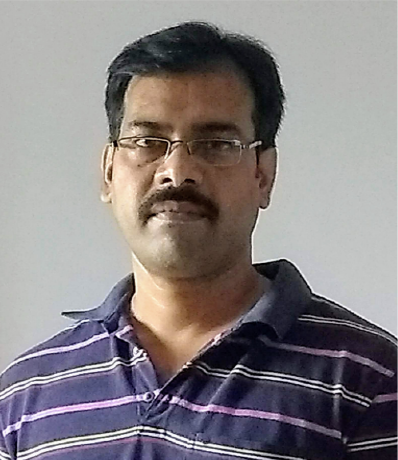
\includegraphics[scale=0.2]{self}%

\end{figure}

Dr. M. Kamakshaiah is a open source software evangelist, full stack developer and academic of data science and anaytics. His teaching interests are IT practices in business, MIS, Data Science, Business Analytics including functional analytics related to marketing, finance, and HRM, quality and operations. He also teaches theoretical concepts like statistical diagnosis, multivariate analytics, numerical simulations \& optimization, machine learning \& AI, IoT using few programming languages like R, Python, Java and more. 

His research interests are related to few domains such as healthcare, education, food \& agriculture, open source software and etc. He has taught abroad for two years and credits two country visits. He has developed few free and open source software solutions meant for corporate practitioners, academics, scholars and students engaging in data science and analytics. All his software applications are available from his GITHUB portal \url{https://github.com/Kamakshaiah}. 

\tableofcontents

\chapter*{Preface}

This book is a result of my teaching necessity. The necessity arose out of dearth of good text book meant for students in business management stream. There are books on C++ but not sufficient enough to address my class room needs. Most of the students in my classes don't have much of programming background and needs exposure to the same having no compromise on coding. 

This text book has five chapters each with a unique goal. This book caters to the needs of both beginners and mavericks. The first chapter deals with introduction to C++ such as history, design principles, few essential components and more. Second chapter deals with few concepts related to code blocks such as data types, operators with related examples. Third chapter deals with control flow consisting code blocks related to conditional statements and loops. The fourth chapter deals with various aspects of Object Oriented Programming (OOP). The last chapter has few code snippets which demonstrates exception handling using C++ in-build methods. 

Most of the examples or code blocks are related to data science and analytics such as arithmetic calculations, less intensive numerical analysis etc., so that even a beginner could pick up content without a doubt. There are few code blocks that are brainy and requires sufficient understanding on core statistics such as statistical tests, methods and modes so on. 

Happy reading ...

\begin{flushright}
	Author \\
	Dr. M. Kamakshaiah
\end{flushright}

\chapter{Introduction}

C++ is a general purpose, case-sensitive, free-form programming language that supports object-oriented, procedural and generic programming. C++ is a middle-level language, as it encapsulates both high and low level language features. C++ supports the object-oriented programming, the four major pillar of object-oriented programming (OOPs) used in C++ are:

\begin{enumerate}
	\item Inheritance
\item Polymorphism
\item Encapsulation
\item Abstraction
\end{enumerate}

Standard C++ programming is divided into three important parts:

\begin{enumerate}
	\item The core library includes the data types, variables and literals, etc.
\item The standard library includes the set of functions manipulating strings, files, etc.
\item The Standard Template Library (STL) includes the set of methods manipulating a data structure.
\end{enumerate}

By the help of C++ programming language, we can develop different types of secured and robust applications:

\begin{enumerate}
	\item Window application
\item Client-Server application
\item Device drivers
\item Embedded firmware etc
\end{enumerate}

\textbf{\textit{C++ Example Program}}

\begin{verbatim}
#include <iostream>  
using namespace std;  
int main() {  
   cout << "Hello C++ Programming";  
   return 0;  
}  
\end{verbatim}

The above program has the sample code that prints a statement \texttt{Hello C++ Programming}. The keyword \texttt{#include} is a C++ keyword which deals with imports. In this program this keyword import one core library called \texttt{iostream}. The second statement deals with namespace, which is a common concept in programming. Every program depends on two very important environmental requirements viz., \texttt{workspace, namespace}. The other keyword \texttt{cout} is \texttt{std} command, which takes care of printing output. The last statement \texttt{return 0}, is required to tell C++ compiler as what is being returned by the method (\texttt{main}, in this case). We will discuss about all these statements in detail through forthcoming sections in this book. 

\section{C vs. C++}

\subsection{What is C?}

C is a structural or procedural oriented programming language which is machine-independent and extensively used in various applications. C is the basic programming language that can be used to develop from the operating systems (like Windows) to complex programs like Oracle database, Git, Python interpreter, and many more. C programming language can be called a god's programming language as it forms the base for other programming languages. If we know the C language, then we can easily learn other programming languages. C language was developed by the great computer scientist \textit{Dennis Ritchie} at the Bell Laboratories. It contains some additional features that make it unique from other programming languages.

\subsection{What is C++?}

C++ is a special-purpose programming language developed by \textit{Bjarne Stroustrup} at Bell Labs circa 1980. C++ language is very similar to C language, and it is so compatible with C that it can run $99\%$ of C programs without changing any source of code though C++ is an object-oriented programming language, so it is safer and well-structured programming language than C.

The following are the differences between C and C++:

\begin{enumerate}
	\item \textit{Definition}: C is a structural programming language, and it does not support classes and objects, while C++ is an object-oriented programming language that supports the concept of classes and objects.
\item \textit{Type of programming language}: C supports the structural programming language where the code is checked line by line, while C++ is an object-oriented programming language that supports the concept of classes and objects.
\item \textit{Developer of the language}: Dennis Ritchie developed C language at Bell Laboratories while Bjarne Stroustrup developed the C++ language at Bell Labs circa 1980.
\item \textit{Subset}: C++ is a superset of C programming language. C++ can run $99\%$ of C code but C language cannot run C++ code.
\item \textit{Type of approach}: C follows the top-down approach, while C++ follows the bottom-up approach. The top-down approach breaks the main modules into tasks; these tasks are broken into sub-tasks, and so on. The bottom-down approach develops the lower level modules first and then the next level modules.
\item \textit{Security}: In C, the data can be easily manipulated by the outsiders as it does not support the encapsulation and information hiding while C++ is a very secure language, i.e., no outsiders can manipulate its data as it supports both encapsulation and data hiding. In C language, functions and data are the free entities, and in C++ language, all the functions and data are encapsulated in the form of objects.
\item \textit{Function Overloading}: Function overloading is a feature that allows you to have more than one function with the same name but varies in the parameters. C does not support the function overloading, while C++ supports the function overloading.
\item \textit{Function Overriding}: Function overriding is a feature that provides the specific implementation to the function, which is already defined in the base class. C does not support the function overriding, while C++ supports the function overriding.
\item \textit{Reference variables}: C does not support the reference variables, while C++ supports the reference variables.
\item \textit{Keywords}: C contains 32 keywords, and C++ supports 52 keywords.
\item \textit{Namespace feature}: A namespace is a feature that groups the entities like classes, objects, and functions under some specific name. C does not contain the namespace feature, while C++ supports the namespace feature that avoids the name collisions.
\item \textit{Exception handling}: C does not provide direct support to the exception handling; it needs to use functions that support exception handling. C++ provides direct support to exception handling by using a \texttt{try-catch} block.
\item \textit{Input/Output functions}: In C, \texttt{scanf} and \texttt{printf} functions are used for input and output operations, respectively, while in C++, \texttt{cin} and \texttt{cout} are used for input and output operations, respectively.
\item \textit{Memory allocation and de-allocation}: C supports \texttt{calloc()} and \texttt{malloc()} functions for the memory allocation, and \texttt{free()} function for the memory de-allocation. C++ supports a new operator for the memory allocation and \texttt{delete} operator for the memory de-allocation.
\item \textit{Inheritance}: Inheritance is a feature that allows the child class to reuse the properties of the parent class. C language does not support the inheritance while C++ supports the inheritance.
\item \textit{Header file}: C program uses \texttt{<stdio.h>} header file while C++ program uses \texttt{<iostream.h>} header file.
\end{enumerate}

\section{C++ history}

History of C++ language is interesting to know. Here we are going to discuss brief history of C++ language. C++ programming language was developed in 1980 by Bjarne Stroustrup at bell laboratories of AT&T (American Telephone & Telegraph), located in U.S.A. Bjarne Stroustrup is known as the founder of C++ language. It was develop for adding a feature of OOP (Object Oriented Programming) in C without significantly changing the C component. C++ programming is \enquote{relative} (called a superset) of C, it means any valid C program is also a valid C++ program. programming languages that were developed before C++ language.

\begin{table}[h]
\centering
\begin{tabular}{lll} \hline 
Language	& Year	& Developed By \\ \hline
Algol	& 1960	& International Group \\
BCPL	& 1967	& Martin Richard \\
B	& 1970	& Ken Thompson \\
Traditional C	& 1972	& Dennis Ritchie \\
K \& R C	& 1978	& Kernighan \& Dennis Ritchie \\ \hline 

\end{tabular}
\caption{Languages that were developed before C++ language}
\label{}
\end{table}

\section{C++ Features}

C++ is object oriented programming language. It provides a lot of features that are given below.

\begin{comment}
\begin{enumerate}
	\item Simple
\item Machine Independent or Portable
\item Mid-level programming language
\item Structured programming language
\item Rich Library
\item Memory Management
\item Fast Speed
\item Pointers
\item Recursion
\item Extensible
\item Object Oriented
\item Compiler based
\end{enumerate}
\end{comment} 

\begin{enumerate}
	\item \textit{Simple}: C++ is a simple language in the sense that it provides structured approach (to break the problem into parts), rich set of library functions, data types etc.

\item \textit{Machine Independent or Portable}: Unlike assembly language, c programs can be executed in many machines with little bit or no change. But it is not platform-independent.

\item \textit{Mid-level programming language}: C++ is also used to do low level programming. It is used to develop system applications such as kernel, driver etc. It also supports the feature of high level language. That is why it is known as mid-level language.

\item \textit{Structured programming language}: C++ is a structured programming language in the sense that we can break the program into parts using functions. So, it is easy to understand and modify.

\item \textit{Rich Library}: C++ provides a lot of inbuilt functions that makes the development fast.

\item \textit{Memory Management}: It supports the feature of dynamic memory allocation. In C++ language, we can free the allocated memory at any time by calling the free() function.

\item \textit{Speed}: The compilation and execution time of C++ language is fast.

\item \textit{Pointer}: C++ provides the feature of pointers. We can directly interact with the memory by using the pointers. We can use pointers for memory, structures, functions, array etc.

\item \textit{Recursion}: In C++, we can call the function within the function. It provides code reusability for every function.

\item \textit{Extensible}: C++ language is extensible because it can easily adopt new features.

\item \textit{Object Oriented}: C++ is object oriented programming language. OOPs makes development and maintenance easier where as in Procedure-oriented programming language it is not easy to manage if code grows as project size grows.

\item \textit{Compiler based}: C++ is a compiler based programming language, it means without compilation no C++ program can be executed. First we need to compile our program using compiler and then we can execute our program.
\end{enumerate}

\section{Installation}

There are number of ways to install and work with C++. Following are few ways: 

\begin{enumerate}
	\item Using CLI. \endnote{Refer to WSL \url{https://docs.microsoft.com/en-us/windows/wsl/about} for more information).} 
	\item POSIX-like run-time environments such as CygWin \& MinGW. \endnote{Refer to \url{https://www.linux.org/threads/introducing-mingw-and-cygwin.11535/}.} \endnote{POSIX stands for \emph{Portable Operating System Interface (POSIX)}. There are few ways to get POSIX based Linux run-time libraries to Windows. Two of the most famous ways is either through MinGW or Cygwin. However, there are umpteen number of portals or sites for these libraries. Two of the most famous things (apart from downloading straight from their respective portals) is either using \url{https://winlibs.com/} or \url{http://win-builds.org/doku.php}. Winlibs is perhaps most straight forward approach for setting up POSIX environments in Windows. }
	
	\item Third party Integrated Development Environments (IDEs). Example: Dev-C++ \endnote{Visit http://www.bloodshed.net/ for information).}
	\item Install C and C++ support in \textit{Visual Studio}. \endnote{Refer to \url{https://docs.microsoft.com/en-us/cpp/build/vscpp-step-0-installation?view=msvc-160} for more information.} 
	\item C/C++ for \textit{Visual Studio Code}. \endnote{Visit \url{https://code.visualstudio.com/docs/languages/cpp} for more information.} 
	\item C++ on Eclipse in Windows. \endnote{Visit \url{https://www.eclipse.org/downloads/packages/release/neon/3/eclipse-ide-cc-developers} for more information. }
\end{enumerate}

I suggest and will be using the last method among all the above methods for it is consistent for many reasons. One of the potential reasons is that Eclipse is an editor for many languages and also support few platforms such as mobile, desktop, web, IoT, etc. So using Eclipse always offers rather more mileage over other methods and editors. 

\subsection{Eclipse for C++}

Eclipse is an integrated development environment (IDE) used in computer programming. It contains a base workspace and an extensible plug-in system for customizing the environment. Eclipse is written mostly in Java and its primary use is for developing Java applications, but it may also be used to develop applications in other programming languages via plug-ins, including Ada, ABAP, C, C++, C\#, Clojure, COBOL, D, Erlang, Fortran, Groovy, Haskell, JavaScript, Julia, Lasso, Lua, Perl, PHP, Prolog, Python, R, Ruby (including Ruby on Rails framework), Rust, Scala, and Scheme. It can also be used to develop documents with LaTeX and packages for the software Mathematica. Development environments include the Eclipse Java development tools (JDT) for Java and Scala, Eclipse CDT for C/C++, and Eclipse PDT for PHP, among others.

\subsubsection{Install MinGW GCC or Cygwin GCC}

To use Eclipse for C/C++ programming, you need a C/C++ compiler. On Windows, you could install either MinGW GCC or Cygwin GCC. Choose MinGW if you are not sure, because MinGW is lighter and easier to install, but has fewer features.

To install MinGW, go to the MinGW homepage, \url{www.mingw.org}, and follow the link to the MinGW download page. Download the latest version of the MinGW installation program which should be named \textit{MinGW$<$version$>$.exe}. While installing MinGW, at a minimum, you must install \textit{gcc-core, gcc-g++, binutils}, and the \textit{MinGW runtime}, but you may wish to install more. \textit{Add the bin subdirectory of your MinGW installation to your PATH environment variable so that you can specify these tools on the command line by their simple names}.

\subsubsection{Install Eclipse C/C++ Development Tool (CDT)}

There are two ways to install CDT, depending on whether you have previously installed an Eclipse. If you have already installed \enquote{Eclipse for Java Developers} or other Eclipse packages, you could install the CDT plug-in as follows. 

\begin{enumerate}
	\item Launch Eclipse -$>$ Help -$>$ Install New Software -$>$ In \enquote{Work with} field, pull down the drop-down menu and select \enquote{Kepler - http://download.eclipse.org/releases/kepler} (or juno for Eclipse 4.2; or helios for Eclipse 3.7).

\item In \enquote{Name} box, expand \enquote{Programming Language} node -$>$ Check \enquote{C/C++ Development Tools} -$>$ \enquote{Next} -$>$ ... -$>$ \enquote{Finish}.
\end{enumerate}

If you have not install any Eclipse package, you could download \enquote{Eclipse IDE for C/C++ Developers} from \url{http://www.eclipse.org/downloads}, and unzip the downloaded file into a directory of your choice.

\subsection{Creating C++ project}

Eclipse has perspectives, this means Eclipse base IDE can be made convenient for a given run-time environment. If you have installed Eclipse CDT (C++ Development Tooling), then you probably don't need to switch between perspectives. If you working with multiple run-times then probably you need to switch between perspectives in Eclipse. There are many ways to switch perspectives in Eclipse. 

\begin{enumerate}
	\item Windows short-cut key combination is \emph{Ctl+F8}. 
	\item There is perspectives button at right upper corner of the Eclipse toolbar. 
	\item Using Eclipse main menu: Window -$>$ Perspectives -$>$ Open Perspective -$>$ Other: C++

\end{enumerate}

Once, you are in CDT perspective then go to File -$>$ Create Project. After finishing necessary formalities like naming folders/files and selecting proper locations for these folders and files, you may find a folder created at left file explorers windows inside Eclipse. Right click on the main (or project home) directory, select New -$>$ \enquote{Source File}. \textbf{Try to save the file with \emph{.cpp} format.} Now you are literally ready for C++ development. \endnote{Inna Pivkina wrote a nice blog on Eclipse perspectives. Visit \url{https://www.cs.nmsu.edu/~ipivkina/cs278/eclipsetutorial.html} for more details.}

\section{C++ Program from terminal}

 First let us understand as how to compile and run C++ files from terminal. Create a nice place, you may call it as workspace, as every programming language need to have certain workspace and namespace for running their code. At times, it can be a simple folder in which we are going to organize our scripts. In my computer I created one such folder and it looks like the one below: 

\begin{verbatim}
D:\Work\Books\CPP\scripts>dir
 Volume in drive D is Data
 Volume Serial Number is 0C88-924D

 Directory of D:\Work\Books\CPP\scripts

24-10-2021  18:20    <DIR>          .
24-10-2021  18:20    <DIR>          ..
24-10-2021  18:19                 0 demo.cpp
               1 File(s)              0 bytes
               2 Dir(s)  659,893,870,592 bytes free

D:\Work\Books\CPP\scripts>
\end{verbatim}

\texttt{D:\Work\Books\CPP\scripts} is the workspace for my C++ programs. If you see I have one file with name \texttt{demo.cpp}. This is the file in which I am going to write C++ program. Let's try the following code snippet in plain text file in Windows known as \emph{Notepad}. 

\begin{verbatim}
#include <iostream>
using namespace std;

int main(){
	cout << "Hello World!" << endl;
	cout << "This is first C++ program.";
	return 0;
}
\end{verbatim}

Now in the terminal use the following statement to compile this program. 

\begin{verbatim}
g++ demo.cpp
\end{verbatim}

This shall produce the following changes in the same directory. 

\begin{verbatim}
D:\Work\Books\CPP\scripts>dir
 Volume in drive D is Data
 Volume Serial Number is 0C88-924D

 Directory of D:\Work\Books\CPP\scripts

24-10-2021  18:25    <DIR>          .
24-10-2021  18:25    <DIR>          ..
24-10-2021  18:25            56,932 a.exe
24-10-2021  18:24               147 demo.cpp
               2 File(s)         57,079 bytes
               2 Dir(s)  659,893,624,832 bytes free
\end{verbatim}

A new file \emph{a.exe} is produced which is an Windows executable file. Now if you run \texttt{a.exe} in the terminal it shall produce the output. 

\begin{verbatim}
D:\Work\Books\CPP\scripts>a.exe
Hello World!
This is first C++ program.
\end{verbatim}

As far as compiling is concerned, there are number of ways to compile a C++ program into variety of output formats. 

\begin{enumerate}
	\item \texttt{g++ -S}: generates a \emph{file\_name.s} known as assembly source file. 
	\item \texttt{g++ -c}: generates a \emph{file\_name.o} object code file in present working directory.
	\item \texttt{g++ -o/exe}: generates executable target file with \texttt{target\_name} (or a.out by default).
\end{enumerate}

Suppose I want to compile to an output file with a given name. I need to execute the same statement with few changes shown as below. 

\begin{verbatim}
g++ -o main.exe demo.cpp
\end{verbatim}

This will create \texttt{main.exe} in the same filder/directory. 

\subsection{Object code}

Object code is highly useful to \emph{compile and link multiple files}. I want to plan my project as below: 

\begin{enumerate}
	\item Create a header (.h) file with method definitions (\texttt{helloworld.h}). 
	\item Define the method (\texttt{helloworld.cpp}). 
	\item Invoke the method from \emph{main} file (\texttt{hello.cpp}). 
\end{enumerate}

So I am planning my project with one header file and two \emph{cpp} files. Keep all the files in the same directory. The code inside these files is going to be as below: 

\begin{verbatim}
// hello.cpp file
#include "helloWorld.h"
#include <iostream>
int main()
{
    std::cout << "This is \n";
    helloWorld();
		std::cout << "greeting"; 
    return 0;
}

// helloWorld.cpp file
#include <iostream>
void helloWorld()
{
    std::cout << "Hello World\n";
}

// helloWorld.h file
void helloWorld();
\end{verbatim}

Now run the following statements in the terminal. 

\begin{verbatim}
g++ -c helloWorld.cpp hello.cpp
g++ -o main.exe hello.o helloworld.o
\end{verbatim}

This shall produce executable file with name \texttt{main.exe}, which can produce the below output.  

\begin{verbatim}
This is
Hello World
greeting 
\end{verbatim}

\section{Eclipse for C++ development}

In the main menu go to File -$>$ New and create Source File, but save the file with \emph{.cpp} extension. This can also be done by right clicking project directory. Eclipse will display a file which is just a normal text file but with \emph{.cpp} extension. Write the following code in it. 

\begin{verbatim}
#include <iostream>
using namespace std;

int main(){
	cout << "Hello World!" << endl;
	cout << "This is first C++ program.";
	return 0;
}
\end{verbatim}

Go to Project -$>$ Build All (Ctl + B). This action shall produce a couple of additional folders and files in those folder. Now go to Run -$>$ Run As -$>$ Local C/C++ Application (Ctl + F11). This shall produce the following output in the Eclipse Console. 

\begin{verbatim}
Hello World!
This is first C++ program.
\end{verbatim}

\section{Basic Input/Output}

C++ I/O operation is using the stream concept. Stream is the sequence of bytes or flow of data. It makes the performance fast. 
If bytes flow from main memory to device like printer, display screen, or a network connection, etc, this is called as output operation. If bytes flow from device like printer, display screen, or a network connection, etc to main memory, this is called as input operation. 

\subsection{I/O Library Header Files}
% https://www.tutorialspoint.com/cplusplus/cpp_files_streams.htm

Let us see the common header files used in C++ programming are:

\begin{comment}
\begin{table}[h]
\begin{tabular}{ll} \hline 
Header File	& Function and Description \\ \hline 
\texttt{<iostream>}	& It is used to define the \\
& \texttt{cout}, \texttt{cin} and \texttt{cerr} objects, which correspond to \\
& standard output stream, standard input stream \\
& and standard error stream, respectively. \\
\texttt{<iomanip>}	& It is used to declare \\
& services useful for performing formatted I/O, \\
& such as \texttt{setprecision} and \texttt{setw}. \\
\texttt{<fstream>}	& It is used to declare \\ 
& services for user-controlled file processing. \\ \hline 
\end{tabular}
\caption{Header files}
\label{}
\end{table}
\end{comment} 

\begin{enumerate}
	\item \texttt{#include<stdio.h>}: It is used to perform input and output operations using functions \texttt{scanf()} and \texttt{printf()}.
\item \texttt{#include<iostream>}: It is used as a stream of Input and Output using \texttt{cin} and \texttt{cout}.
\item \texttt{#include<string.h>}: It is used to perform various features related to string manipulation like \texttt{strlen(), strcmp(), strcpy(), size()}, etc.
\item \texttt{#include<math.h>}: It is used to perform mathematical operations like \texttt{sqrt(), log2(), pow()}, etc.
\item \texttt{#include<iomanip.h>}: It is used to access \texttt{setw()} and \texttt{setprecision()} function to limit the decimal places in variables.
\item \texttt{#include<signal.h>}: It is used to perform signal handling functions like \texttt{signal()} and \texttt{raise()}.
\item \texttt{#include<stdarg.h>}:It is used to perform standard argument functions like \texttt{va\_start()} and \texttt{va\_arg()}. It is also used to indicate start of the variable-length argument list and to fetch the arguments from the variable-length argument list in the program respectively.
\item \texttt{#include<errno.h>}: It is used to perform error handling operations like \texttt{errno(), strerror(), perror()}, etc.
\item \texttt{#include<fstream.h>}: It is used to control the data to read from a file as an input and data to write into the file as an output.
\item \texttt{#include<time.h>}: It is used to perform functions related to \texttt{date()} and \texttt{time()} like \texttt{setdate()} and \texttt{getdate()}. It is also used to modify the system date and get the CPU time respectively.
\item \texttt{#include<float.h>}: It contains a set of various platform-dependent constants related to floating point values. These constants are proposed by ANSI C. They allow making programs more portable. Some examples of constants included in this header file are- e(exponent), b(base/radix), etc.
\item \texttt{#include<limits.h>}: It determines various properties of the various variable types. The macros defined in this header, limits the values of various variable types like char, int, and long. These limits specify that a variable cannot store any value beyond these limits, for example an unsigned character can store up to a maximum value of 255.
\end{enumerate}


\subsection{Standard output stream (\texttt{cout})}

The \texttt{cout} is a predefined object of \texttt{ostream} class. It is connected with the standard output device, which is usually a display screen. The \texttt{cout} is used in conjunction with stream insertion operator ($<<$) to display the output on a console. Let's see the simple example of standard output stream (\texttt{cout}):

\begin{verbatim}
#include <iostream>  
using namespace std;  
int main( ) {  
   char ary[] = "Welcome to C++ tutorial";  
   cout << "Value of ary is: " << ary << endl;  
}  
\end{verbatim}

Output:
\begin{verbatim}
Value of ary is: Welcome to C++ tutorial
\end{verbatim}

\subsection{Standard input stream (\texttt{cin})}

The \texttt{cin} is a predefined object of \texttt{istream} class. It is connected with the standard input device, which is usually a keyboard. The \texttt{cin} is used in conjunction with stream extraction operator ($>>$) to read the input from a console. Let's see the simple example of standard input stream (\texttt{cin}):

\begin{verbatim}
#include <iostream>  
using namespace std;  
int main( ) {  
  int age;  
   cout << "Enter your age: ";  
   cin >> age;  
   cout << "Your age is: " << age << endl;  
}  
\end{verbatim} 

Output:
\begin{verbatim}
Enter your age: 22
Your age is: 22
\end{verbatim}

\subsection{Standard end line (\texttt{endl})}

The \texttt{endl} is a predefined object of \texttt{ostream} class. It is used to insert a new line characters and flushes the stream. Let's see the simple example of standard end line (\texttt{endl}):

\begin{verbatim}
#include <iostream>  
using namespace std;  
int main( ) {  
cout << "C++ Tutorial";     
cout << " Javatpoint"<<endl;   
cout << "End of line"<<endl;   
}   
\end{verbatim}

Output:
\begin{verbatim}
C++ Tutorial Javatpoint 
End of line
\end{verbatim}

\section{Identifiers and Keywords}

\subsection{Identifiers}

C++ identifiers in a program are used to refer to the name of the \emph{variables, functions, arrays}, or other \emph{user-defined data types} created by the programmer. They are the basic requirement of any language. Every language has its own rules for naming the identifiers. In short, we can say that the C++ identifiers represent the essential elements in a program which are given below:

\begin{enumerate}
	\item Constants
\item Variables
\item Functions
\item Labels
\item Defined data types
\end{enumerate}

\subsection{Naming rules}

\begin{enumerate}
	\item Only alphabetic characters, digits, and underscores are allowed.
\item The identifier name cannot start with a digit, i.e., the first letter should be alphabetical. After the first letter, we can use letters, digits, or underscores.
\item In C++, uppercase and lowercase letters are distinct. Therefore, we can say that C++ identifiers are case-sensitive.
\item A declared keyword cannot be used as a variable name.
\end{enumerate}

For example, suppose we have two identifiers, named as 'FirstName', and 'Firstname'. Both the identifiers will be different as the letter 'N' in the first case in uppercase while lowercase in second. Therefore, it proves that identifiers are case-sensitive. Following are few valid Identifiers

\begin{enumerate}
	\item Result  
\item Test2  
\item \_sum  
\item power 
\end{enumerate}

The following are the examples of invalid identifiers:

\begin{enumerate}
	\item Sum-1   // containing special character '-'.  
\item 2data    // the first letter is a digit.   
\item break    // use of a keyword.    
\end{enumerate}

The major difference between C and C++ is the limit on the length of the name of the variable. ANSI C considers only the first 32 characters in a name while ANSI C++ imposes no limit on the length of the name. Constants are the identifiers that refer to the fixed value, which do not change during the execution of a program. Both C and C++ support various kinds of literal constants, and they do have any memory location. For example, 123, 12.34, 037, 0X2, etc. are the literal constants. Let's look at a simple example to understand the concept of identifiers.

\begin{lstlisting}
#include <iostream>  
using namespace std;  
int main()  
{  
	int a;  
	int A;  
	cout<<"Enter the values of 'a' and 'A'";  
	cin>>a;  
	cin>>A;  
	cout<<"\nThe values that you have entered are : "<<a<<" , "<<A;  
	return 0;  
}  
\end{lstlisting}

In the above code, we declare two variables 'a' and 'A'. Both the letters are same but they will behave as different identifiers. As we know that the identifiers are the case-sensitive so both the identifiers will have different memory locations.

\subsection{Keywords}

Keywords are the reserved words that have a special meaning to the compiler. They are reserved for a special purpose, which cannot be used as the identifiers. For example, 'for', 'break', 'while', 'if', 'else', etc. are the predefined words where predefined words are those words whose meaning is already known by the compiler. Whereas, the identifiers are the names which are defined by the programmer to the program elements such as variables, functions, arrays, objects, classes.

Table \ref{keywords} has the list of all C++ keywords. (as of C++17)

\begin{table}[h]
\centering 
\begin{tabular}{llll} \hline 
alignas	& decltype	& namespace	& struct \\
alignof	& default	& new	& switch \\
and	& delete	& noexcept	& template \\
and\_eq	& do	& not	& this \\
asm	& double	& not\_eq	& thread\_local \\
auto	& dynamic\_cast &	nullptr	& throw \\
bitand	& else	& operator	& true \\
bitor	& enum	& or	& try \\
bool	& explicit	& or\_eq	& typedef \\
break	& export	& private	& typeid \\
case	& extern	& protected	& typename \\
catch	& false	& public	& union \\
char	& float	& register	& unsigned \\
char16\_t	& for	& reinterpret\_cast	& using \\
char32\_t	& friend	& return	& virtual \\
class	& goto	& short	& void \\
compl	& if	& signed	& volatile \\
const	& inline	& sizeof	& wchar\_t \\
constexpr	& int	& static	& while \\
const\_cast	& long	& static\_assert	& xor \\
continue	& mutable	& static\_cast	& xor\_eq \\ \hline 
\end{tabular}
\caption{Keywords in C++}
\label{keywords}
\end{table}

The Table \ref{identifiersandkeywords} has the list of differences between identifiers and keywords:

\begin{table}[h]
\centering 
\begin{tabular}{ll} \hline 
Identifiers	& Keywords \\ \hline 
Identifiers are the names  &	Keywords are the reserved  \\
defined by the programmer  & words whose meaning is known \\ 
to the basic elements of a &  by the compiler. \\
program.										& \\ \hline 
It is used to identify the 	& It is used to specify the  \\ 
name of the variable. &  type of entity. \\ \hline 
It can consist of letters, 	& It contains only letters. \\ 
digits, and underscore. & \\ \hline 
It can use both lowercase & It uses only lowercase letters. \\ 
and uppercase letters. & \\ \hline 
No special character can 	& It cannot contain any  \\ 
be used except the underscore. & special character. \\ \hline
The starting letter of  & 	It can be started only with  \\
identifiers can be lowercase,  & the lowercase letter. \\ 
uppercase or underscore. & \\ \hline 
It can be classified as 	& It cannot be further classified. \\ 
internal and external identifiers. & \\ \hline 
Examples are test, result, 	& Examples are 'for', 'if',  \\  
sum, power, etc. & 'else', 'break', etc. \\ \hline
\end{tabular}
\caption{Differences between identifiers and keywords.}
\label{identifiersandkeywords}
\end{table}

\section{Data Types}

All variables use data-type during declaration to restrict the type of data to be stored. Therefore, we can say that data types are used to tell the variables the type of data it can store. Whenever a variable is defined in C++, the compiler allocates some memory for that variable based on the data-type with which it is declared. Every data type requires a different amount of memory.

\begin{figure}[h]
\centering 
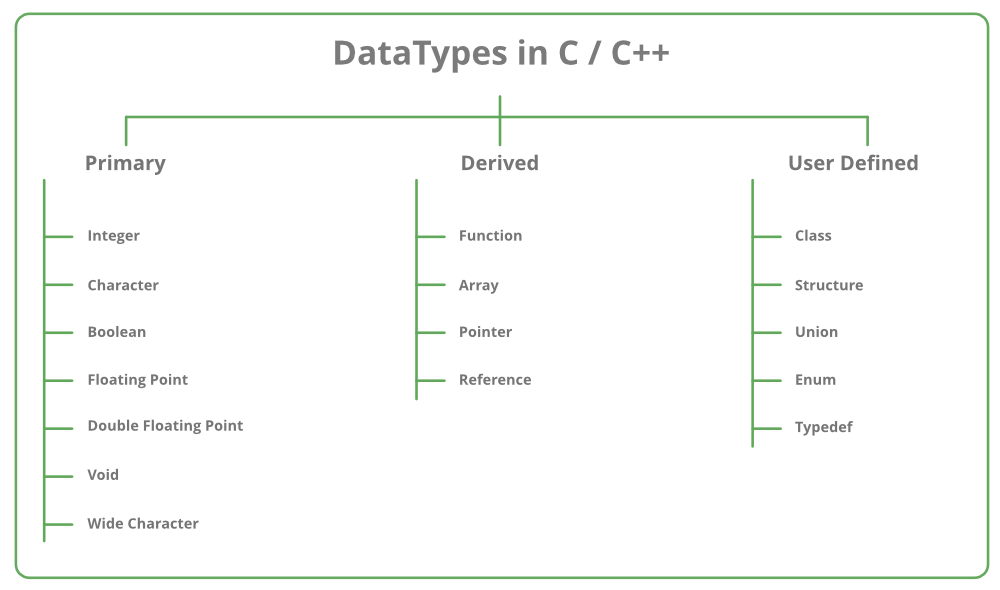
\includegraphics[width=9cm, height=5cm]{datatypesinc}%
\caption{Data types in C}%
\label{}%
\end{figure}

A data type specifies the type of data that a variable can store such as integer, floating, character etc. There are 4 types of data types in C++ language. Data types in C++ is mainly divided into three types: 

\begin{enumerate}
	\item \textbf{Primitive Data Types:} These data types are built-in or predefined data types and can be used directly by the user to declare variables. example: int, char , float, bool etc. Primitive data types available in C++ are: 
	\begin{itemize}
		\item Integer
\item Character
\item Boolean
\item Floating Point
\item Double Floating Point
\item Valueless or Void
\item Wide Character
\end{itemize}

\item \textbf{Derived Data Types:} The data-types that are derived from the primitive or built-in datatypes are referred to as Derived Data Types. These can be of four types namely: 
\begin{itemize}
	\item Function
\item Array
\item Pointer
\item Reference
\end{itemize}
\item \textbf{Abstract or User-Defined Data Types:} These data types are defined by user itself. Like, defining a class in C++ or a structure. C++ provides the following user-defined datatypes: 
\begin{itemize}
	\item Class
\item Structure
\item Union
\item Enumeration
\item Typedef defined DataType
\end{itemize}
\end{enumerate}



\begin{comment}
\begin{table}[h]
\begin{tabular}{ll} \hline 
Types	& Data Types \\ \hline
Basic Data Type	& int, char, float, double, etc \\
Derived Data Type	& array, pointer, etc \\
Enumeration Data Type	& enum \\
User Defined Data Type	& structure \\ \hline 
\end{tabular}
\caption{Data types}
\label{}
\end{table}
\end{comment} 

\subsection{Basic Data Types}

The basic data types are integer-based and floating-point based. C++ language supports both signed and unsigned literals. 
The memory size of basic data types may change according to 32 or 64 bit operating system. Let's see the basic data types. It size is given according to 32 bit OS.

\begin{enumerate}
	\item \textbf{Integer:} Keyword used for integer data types is int. Integers typically requires 4 bytes of memory space and ranges from -2147483648 to 2147483647. 
 
\item \textbf{Character}: Character data type is used for storing characters. Keyword used for character data type is char. Characters typically requires 1 byte of memory space and ranges from -128 to 127 or 0 to 255. 
 
\item \textbf{Boolean}: Boolean data type is used for storing boolean or logical values. A boolean variable can store either true or false. Keyword used for boolean data type is bool. 
 
\item \textbf{Floating Point}: Floating Point data type is used for storing single precision floating point values or decimal values. Keyword used for floating point data type is float. Float variables typically requires 4 byte of memory space. 
 
\item \textbf{Double Floating Point:} Double Floating Point data type is used for storing double precision floating point values or decimal values. Keyword used for double floating point data type is double. Double variables typically requires 8 byte of memory space. 
 
\item \textbf{void:} Void means without any value. void datatype represents a valueless entity. Void data type is used for those function which does not returns a value. 
 
\item \textbf{Wide Character}: Wide character data type is also a character data type but this data type has size greater than the normal 8-bit datatype. Represented by wchar\_t. It is generally 2 or 4 bytes long. 
\end{enumerate}

The Table \ref{datatypes} shows the tabular representation for above description. 

\begin{table}[h]
\centering 
\begin{tabular}{lll} \hline 
Data Types	& Memory Size	& Range \\ \hline 
char	& 1 byte	& -128 to 127 \\
signed char	& 1 byte	& -128 to 127 \\
unsigned char	& 1 byte	& 0 to 127 \\
short	& 2 byte	& -32,768 to 32,767 \\
signed short	& 2 byte	& -32,768 to 32,767 \\
unsigned short	& 2 byte	& 0 to 32,767 \\
int	& 2 byte	& -32,768 to 32,767 \\
signed int	& 2 byte	& -32,768 to 32,767 \\
unsigned int	& 2 byte	& 0 to 32,767 \\
short int	& 2 byte	& -32,768 to 32,767 \\
signed short int	& 2 byte	& -32,768 to 32,767 \\
unsigned short int	& 2 byte	& 0 to 32,767 \\
long int	& 4 byte & \\
signed long int	& 4 byte & \\
unsigned long int	& 4 byte & \\
float	& 4 byte & \\ 
double	& 8 byte & \\
long double	& 10 byte & \\ \hline 
\end{tabular}
\caption{Basic data types}
\label{datatypes}
\end{table}

\subsection{Datatype Modifiers}
% https://www.oreilly.com/library/view/c-cookbook/0596007612/ch03s08.html
% https://www.cplusplus.com/reference/limits/numeric_limits/

As the name implies, data type modifiers are used with the built-in data types to modify the length of data that a particular data type can hold. 

\begin{figure}[h]
\centering
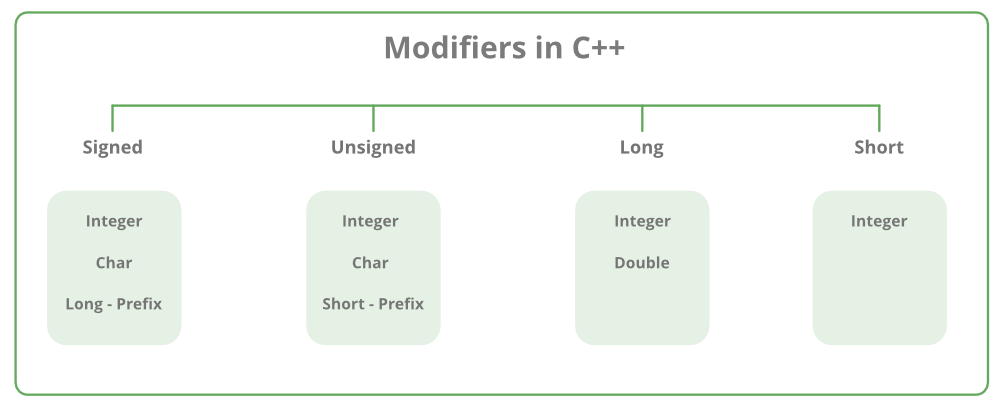
\includegraphics[width=9cm, height=4cm]{modifiers}%
\caption{Modifiers}%
\label{}%
\end{figure}

Data type modifiers available in C++ are:

\begin{enumerate}
	\item Signed
\item Unsigned
\item Short
\item Long
\end{enumerate}

Table \ref{datatypes} summarizes the modified size and range of built-in data types when combined with the type modifiers. These values may vary from compiler to compiler. Values in the above example corresponds to GCC 32 bit. However, it is possible to display the size of all the data types by using the \texttt{sizeof()} operator and passing the keyword of the data type as argument to this function as shown below: 

\begin{lstlisting}
// C++ program to sizes of data types
#include<iostream>
using namespace std;
 
int main()
{
	cout << "Size of char : " << sizeof(char)
		<< " byte" << endl;
	cout << "Size of int : " << sizeof(int)
		<< " bytes" << endl;
	cout << "Size of short int : " << sizeof(short int)
		<< " bytes" << endl;
	cout << "Size of long int : " << sizeof(long int)
		 << " bytes" << endl;
	cout << "Size of signed long int : " << sizeof(signed long int)
		 << " bytes" << endl;
	cout << "Size of unsigned long int : " << sizeof(unsigned long int)
		 << " bytes" << endl;
	cout << "Size of float : " << sizeof(float)
		 << " bytes" <<endl;
	cout << "Size of double : " << sizeof(double)
		 << " bytes" << endl;
	cout << "Size of wchar_t : " << sizeof(wchar_t)
		 << " bytes" <<endl;
	 
	return 0;
}
\end{lstlisting}

Output: 

\begin{lstlisting}
Size of char : 1 byte
Size of int : 4 bytes
Size of short int : 2 bytes
Size of long int : 8 bytes
Size of signed long int : 8 bytes
Size of unsigned long int : 8 bytes
Size of float : 4 bytes
Size of double : 8 bytes
Size of wchar\_t : 4 bytes
\end{lstlisting}

\section{C++ Variables, Literals and Constants}

\subsection{C++ Variables}

In programming, a variable is a container (storage area) to hold data. To indicate the storage area, each variable should be given a unique name (identifier). For example,

\begin{verbatim}
int age = 14;
\end{verbatim}

Here, \texttt{age} is a variable of the \texttt{int} data type, and we have assigned an integer value 14 to it. he \texttt{int} data type suggests that the variable can only hold integers. Similarly, we can use the \texttt{double} data type if we have to store decimals and exponential. The value of a variable can be changed, hence the name variable.

\begin{verbatim}
int age = 14;   // age is 14
age = 17;       // age is 17
\end{verbatim}

\subsection{Rules for naming a variable}

\begin{enumerate}
	\item A variable name can only have alphabets, numbers, and the underscore \_.
\item A variable name cannot begin with a number.
\item Variable names should not begin with an uppercase character.
\item A variable name cannot be a keyword. For example, int is a keyword that is used to denote integers.
\item A variable name can start with an underscore. However, it's not considered a good practice.
\end{enumerate}

\subsection{C++ Literals}

Literals are data used for representing \textit{fixed values}. They can be used directly in the code. For example: 1, 2.5, 'c' etc. Here, 1, 2.5 and 'c' are literals. Why? You cannot assign different values to these terms. Here's a list of different literals in C++ programming.

\begin{enumerate}
	\item \textbf{Integers:} \\
	An integer is a numeric literal(associated with numbers) without any fractional or exponential part. There are three types of integer literals in C programming:
	\begin{itemize}
		\item decimal (base 10)
\item octal (base 8)
\item hexadecimal (base 16)
	\end{itemize}
	In C++ programming, octal starts with a 0, and hexadecimal starts with a 0x.

\item \textbf{Floating-point Literals:} \\
A floating-point literal is a numeric literal that has either a fractional form or an exponent form. For example:
-2.0; 0.0000234; -0.22E-5 (E-5 = 10-5)
\item \textbf{Characters:} \\
A character literal is created by enclosing a single character inside single quotation marks. For example: 'a', 'm', 'F', '2', '\}' etc.
\item \textbf{Escape Sequences: }
Sometimes, it is necessary to use characters that cannot be typed or has special meaning in C++ programming. For example, newline (enter), tab, question mark, etc. In order to use these characters, escape sequences are used.

\begin{table}[h]
\centering 
\begin{tabular}{ll} \hline 
Escape Sequences	& Characters \\ \hline 
\textbackslash b	& Backspace \\
\textbackslash f	& Form feed \\
\textbackslash n	& Newline \\
\textbackslash r	& Return \\
\textbackslash t	& Horizontal tab \\
\textbackslash v	& Vertical tab \\
\textbackslash \$	& Backslash \\
\textbackslash \'	& Single quotation mark \\
\textbackslash \"	& Double quotation mark \\
\textbackslash ?	& Question mark \\
\textbackslash 0	& Null Character \\ \hline 
\end{tabular}
\caption{Escape characters}
\label{}
\end{table}


\item \textbf{String Literals: }
A string literal is a sequence of characters enclosed in double-quote marks. For example:

\begin{table}[h]
\centering
\begin{tabular}{ll} \hline 
"good"	& string constant \\
""	& null string constant \\
" "	& string constant of six white space \\
"x"	& string constant having a single character \\
"Earth is round\n"	& prints string with a newline \\ \hline 
\end{tabular}
\caption{String literals}
\label{}
\end{table}
\end{enumerate}

\subsection{C++ Constants}

In C++, we can create variables whose value cannot be changed. For that, we use the \texttt{const} keyword. Here's an example:

\begin{verbatim}
const int LIGHT\_SPEED = 299792458;
LIGHT\_SPEED = 2500 // Error! LIGHT_SPEED is a constant.
\end{verbatim}

Here, we have used the keyword \texttt{const} to declare a constant named $LIGHT\_SPEED$. If we try to change the value of $LIGHT\_SPEED$, we will get an error.

\section{Operators and Expressions}

C++ expression consists of operators, constants, and variables which are arranged according to the rules of the language. It can also contain function calls which return values. Operators are the foundation of any programming language. Thus the functionality of the C/C++ programming language is incomplete without the use of operators. We can define operators as symbols that help us to perform specific mathematical and logical computations on operands. In other words, we can say that an operator operates the operands. An expression can consist of one or more operands, zero or more operators to compute a value. Every expression produces some value which is assigned to the variable with the help of an assignment operator.

\subsection{Operators}

An operator is a symbol that tells the compiler to perform specific mathematical or logical manipulations. C++ is rich in built-in operators and provide the following types of operators. 

\begin{enumerate}
	\item Arithmetic Operators
\item Relational Operators
\item Logical Operators
\item Bitwise Operators
\item Assignment Operators
\item Misc Operators
\end{enumerate}

This chapter will examine the arithmetic, relational, logical, bitwise, assignment and other operators one by one.

\subsubsection{Arithmetic Operators}

There are following arithmetic operators (Table \ref{arithop}) supported by C++ language. Assume variable A holds 10 and variable B holds 20, then

\begin{table}[h]
\tiny
\centering 
\begin{tabular}{lll} \hline 
Operator	& Description	& Example \\ \hline 
+	& Adds two operands	& A + B will give 30 \\
-	& Subtracts second operand  	& A - B will give -10 \\
& from the first & \\
*	& Multiplies both operands	& A * B will give 200 \\
\/	& Divides numerator by & B / A will give 2 \\
& de-numerator	 & \\
\%	& Modulus Operator and  & B \% A will give 0 \\
& remainder of after an 	 & \\
++	& Increment operator,  	& A++ will give 11 \\
& increases integer division & \\
& integer value by one & \\
$--$	& Decrement operator,  	& A$--$ will give 9 \\ 
& decreases integer value by  & \\ 
& one. & \\ \hline 
\end{tabular}
\caption{}
\label{arithop}
\end{table}

\subsubsection{Relational Operators}

There are following (Table \ref{relop}) relational operators supported by C++ language. Assume variable A holds 10 and variable B holds 20, then

\begin{table}[h]
\tiny
\centering 
\begin{tabular}{lll} \hline 
Operator & Description	& Example \\ \hline 
$==$ &	Checks if the values of  &	(A == B) is not true. \\
& two operands are equal or not,  & \\
& if yes then condition becomes  & \\
& true. & \\
$!=$	& Checks if the values of  &	(A $!=$ B) is true. \\
& two operands are equal or not, & \\
& if values are not equal then  & \\
& condition becomes true. & \\ 
$>$ & Checks if the value of  & (A $>$ B) is not true. \\
& left operand is greater than  & \\
& the value of right operand,  & \\
& if yes then condition becomes true. & \\
$<$ &	Checks if the value of  &	(A $<$ B) is true. \\
& left operand is less than the  & \\
& value of right operand, if yes  & \\
& then condition becomes true. & \\
$>=$	& Checks if the value of  &	(A $>=$ B) is not true. \\
& left operand is greater than or  & \\
& equal to the value of right operand, & \\
&  if yes then condition becomes true. & \\
$<=$	& Checks if the value of left  & (A $<=$ B) is true.\\
& operand is less than or equal  & \\
& to the value of right operand,  & \\ 
& if yes then condition becomes true. & \\ \hline 
\end{tabular}
\caption{Relational operators}
\label{relop}
\end{table}

\subsubsection{Logical operators}

There are following logical operators (Table \ref{logop}) supported by C++ language. Assume variable A holds 1 and variable B holds 0, then

\begin{table}[h]
\tiny
\centering 
\begin{tabular}{lll} \hline \\ 
Operator	& Description	& Example \\ \hline 
$\&\&$ &	Called Logical AND operator. &	(A $\&\&$ B) is false. \\
& If both the operands are non-zero,  & \\
& then condition becomes true. & \\
$||$ &	Called Logical OR Operator. &(A $||$ B) is true. \\
& If any of the two operands is & \\
& non-zero, then condition becomes true. & \\
$!$ &	Called Logical NOT Operator. &	$!(A \&\& B)$ is true. \\
& Use to reverses the logical state of its & \\
& operand. If a condition is true, then & \\
& Logical NOT operator will make false. & \\ \hline 
\end{tabular}
\caption{Logical operators}
\label{logop}
\end{table}

\subsubsection{Bitwise Operators}

Bitwise operator works on bits and perform bit-by-bit operation. The truth tables for $\&, \|,$ and $\^$ are as follows (Table \ref{bitwop})

\begin{table}[h]

\centering 
\begin{tabular}{lllll} \hline \\
p	& q	& $p \& q$ &	$p \| q$ &	$p \^ q$  \\ \hline 
0	& 0	& 0	& 0	& 0 \\
0	& 1	& 0	& 1	& 1 \\
1	& 1	& 1	& 1	& 0 \\
1	& 0	& 0	& 1	& 1 \\ \hline 
\end{tabular}
\caption{Bitwise operators}
\label{bitwop}
\end{table}

Assume if A = 60; and B = 13; now in binary format they will be as follows


A = 0011 1100
B = 0000 1101
-----------------
$A\&B$ = 0000 1100
$A\|B$ = 0011 1101
$A\^B$ = 0011 0001
$\~A$  = 1100 0011

The Bitwise operators supported by C++ language are listed in the following table \ref{bitoper}. Assume variable A holds 60 and variable B holds 13, then

\begin{table}[h]
\tiny
\centering 
\begin{tabular}{lll} \hline \\
Operator	& Description	& Example \\ \hline 
$\&$	& Binary AND Operator copies a &	(A $\&$ B) will give  \\
& bit to the result if it exists in & 12 which is 0000 1100 \\
& both operands. & \\
$|$	& Binary OR Operator copies &	(A $|$ B) will give 61  \\
& a bit if it exists in either operand. & which is 0011 1101 \\
$\hat{} $	& Binary XOR Operator copies &	(A $\hat{}$ B) will give 49  \\
& the bit if it is set in one & which is 0011 0001 \\
& operand but not both. & \\
$\tilde{}$	& Binary Ones Complement Operator &	($\tilde{}A$ ) will give \\
& is unary and has the effect of  & -61 which is 1100 0011 \\
& 'flipping' bits. & in 2's complement form due to a \\
& & signed binary number. \\
$<<$	& Binary Left Shift Operator. &	A << 2 will give  \\
& The left operands value is moved & 240 which is 1111 0000 \\
& left by the number of bits specified  & \\
& by the right operand. & \\
$>>$	& Binary Right Shift Operator. & A >> 2 will give 15  \\
& The left operands value is moved  & which is 0000 1111 \\
& right by the number of bits  & \\
& specified by the right operand. & \\ \hline 

\end{tabular}
\caption{Bitwise operators}
\label{bitoper}
\end{table}

\subsubsection{Assignment Operators}

There are following assignment operators supported by C++ language (Table \ref{assignop}). 

\begin{table}[h]
\tiny
\centering 
\begin{tabular}{lll} \hline \\
Operator	& Description	& Example \\ \hline 
$=$ &	Simple assignment operator, &	C = A + B will  \\
& Assigns values from right side & assign value of A + B into C. \\
& operands to left side operand.  & \\
$+=$ &	Add AND assignment operator, & C += A is  \\
& It adds right operand to the left & equivalent to C = C + A\\
& operand and assign the result  & \\
& to left operand. & \\
$-=$	& Subtract AND assignment operator, &	C -= A is  \\
& It subtracts right operand from  & equivalent to C = C - A \\
& the left operand and assign the result & \\
& to left operand. & \\
$*=$ & Multiply AND assignment operator, &	C *= A is  \\
& It multiplies right operand with  & equivalent to C = C * A \\
& the left operand and assign the  & \\
& result to left operand. & \\
$/=$ &	Divide AND assignment operator, &	C /= A is  \\
& It divides left operand with  & equivalent to C = C / A \\
& the right operand and assign the  & \\
& result to left operand. & \\
$\%=$	& Modulus AND assignment operator, &	C $\%=$ A is  \\
& It takes modulus using two operands  & equivalent to C = C \% A \\
& and assign the result to left operand. & \\
$<<=$ & 	Left shift AND assignment 	& C <<= 2  \\
& operator. &  is same as C = C << 2 \\
$>>=$ & Right shift AND assignment & C >>= 2 is same  \\
& operator. & as C = C >> 2 \\
$\&=$ &	Bitwise AND assignment operator.	& C $\&=$ 2 is \\
& & same as C = C \& 2 \\
$\hat{}=$	& Bitwise exclusive OR and & 	C ^= 2  \\
& assignment operator. & is same as C = C ^ 2 \\
$|=$	& Bitwise inclusive OR and & C |= 2 is same as C = C | 2 \\
& assignment operator. & \\ \hline 
\end{tabular}
\caption{Assignment operator}
\label{assignop}
\end{table}

\subsubsection{Misc Operators}

The following table lists some other operators that C++ supports.

\begin{enumerate}
	\item \texttt{sizeof} \\
sizeof operator returns the size of a variable. For example, \texttt{sizeof(a)}, where ‘a’ is integer, and will return 4.

\item \texttt{Condition ? X : Y} \\
Conditional operator (?). If Condition is true then it returns value of X otherwise returns value of Y.

\item \texttt{,} \\
Comma operator causes a sequence of operations to be performed. The value of the entire comma expression is the value of the last expression of the comma-separated list.

\item . (dot) and -$>$ (arrow) \\
Member operators are used to reference individual members of classes, structures, and unions.

\item \texttt{Cast} \\
Casting operators convert one data type to another. For example, \texttt{int(2.2000)} would return 2.

\item \texttt{\&} \\
Pointer operator $\&$ returns the address of a variable. For example $\&a$; will give actual address of the variable.

\item \texttt{*} \\
Pointer operator \texttt{*} is pointer to a variable. For example \texttt{*var}; will pointer to a variable var.
\end{enumerate}

\subsubsection{Operators Precedence in C++}

Operator precedence determines the grouping of terms in an expression. This affects how an expression is evaluated. Certain operators have higher precedence than others; for example, the multiplication operator has higher precedence than the addition operator. For example x = 7 + 3 * 2; here, x is assigned 13, not 20 because operator * has higher precedence than +, so it first gets multiplied with 3*2 and then adds into 7. Here, operators with the highest precedence appear at the top of the table, those with the lowest appear at the bottom. Within an expression, higher precedence operators will be evaluated first.

\begin{table}[h]
\tiny
\centering 
\begin{tabular}{lll} \hline \\
Category 	& Operator 	& Associativity  \\ \hline 
Postfix 	& $() [] -> . ++ - -$  &	Left to right \\
Unary 	& $+ - ! \tilde{} ++ - -$ (type)* \& sizeof 	& Right to left \\
Multiplicative  &	\& $* \/ \%$ 	& Left to right \\
Additive  	& $+ - $ & Left to right \\
Shift  	& $<< >>$ &	Left to right \\
Relational  &	$< <= > >=$ &	Left to right \\
Equality  &	$== != $ &	Left to right \\
Bitwise AND &	\& 	& Left to right \\
Bitwise XOR &	\hat{} &Left to right \\
Bitwise OR 	& $|$ &	Left to right \\
Logical AND 	& $\&\&$ &	Left to right \\
Logical OR 	& $||$ & 	Left to right \\
Conditional &	$?:$ & 	Right to left  \\
Assignment 	& $= += -= *= /= $ & 	Right to left  \\
& $\%=>>= <<= \&= \hat{}= |=$ & \\
Comma 	& , &	Left to right \\ \hline 

\end{tabular}
\caption{Operator precedence}
\label{}
\end{table}

\subsection{C++ Expression}

An expression is a combination of operators, constants and variables. An expression may consist of one or more operands, and zero or more operators to produce a value.

\begin{figure}[h]
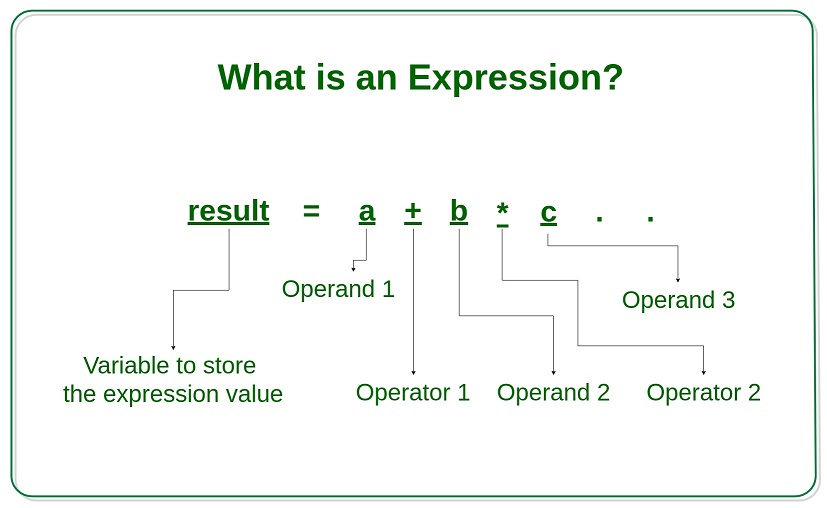
\includegraphics[width=\columnwidth]{expressions}%
\caption{}%
\label{}%
\end{figure}

An expression can be of following types

\begin{enumerate}
	\item Constant expressions
\item Integral expressions
\item Float expressions
\item Pointer expressions
\item Relational expressions
\item Logical expressions
\item Bitwise expressions
\item Special assignment expressions
\end{enumerate}

If the expression is a combination of the above expressions, such expressions are known as \textit{compound expressions}.

\subsubsection{Constant expressions}

A constant expression is an expression that consists of only constant values. It is an expression whose value is determined at the compile-time but evaluated at the run-time. It can be composed of integer, character, floating-point, and enumeration constants. Constants are used in the following situations:

\begin{enumerate}
	\item It is used in the \textit{subscript declarator} to describe the array bound.
\item It is used after the case keyword in the switch statement.
\item It is used as a numeric value in an enum
\item It specifies a bit-field width.
\item It is used in the pre-processor \texttt{#if}
\item In the above scenarios, the constant expression can have integer, character, and enumeration constants. We can use the \item static and \texttt{extern} keyword with the constants to define the function-scope.

\end{enumerate}

The following table shows the expression containing constant value:

\begin{table}[h]
\centering 
\begin{tabular}{ll} \hline 
Expression containing constant	& Constant value \\ \hline 
$x = (2/3) * 4$	& $(2/3) * 4$ \\
$extern int y = 67$	& 67 \\
$int z = 43$	& 43 \\
$static int a = 56$	& 56 \\ \hline 

\end{tabular}
\caption{Expressions }
\label{}
\end{table}

Let's see a simple program containing constant expression:

\begin{lstlisting}
#include <iostream>  
using namespace std;  
int main()  
{  
	int x;        // variable declaration.  
	x=(3/2) + 2;  // constant expression  
	cout<<"Value of x is : "<<x;  // displaying the value of x.  
	return 0;  
}  
\end{lstlisting}

% https://www.javatpoint.com/cpp-expression
In the above code, we have first declared the 'x' variable of integer type. After declaration, we assign the simple constant expression to the 'x' variable.

Output

\begin{Verbatim}
Value of x is : 3  
\end{Verbatim} 

\subsubsection{Integral Expressions}

An integer expression is an expression that produces the integer value as output after performing all the explicit and implicit conversions. Following are the examples of integral expression:

\begin{lstlisting}
(x * y) -5        
x + int(9.0)  
where x and y are the integers.  
\end{lstlisting}

Let's see a simple example of integral expression:

\begin{lstlisting}
#include <iostream>  
using namespace std;  
int main()  
{  
	int x;  // variable declaration.  
	int y;  // variable declaration  
	int z;  // variable declaration  
	cout<<"Enter the values of x and y";  
	cin>>x>>y;  
	z=x+y;  
	cout<<"\n"<<"Value of z is :"<<z; //  displaying the value of z.  
	return 0;  
}  
\end{lstlisting}

In the above code, we have declared three variables, i.e., x, y, and z. After declaration, we take the user input for the values of 'x' and 'y'. Then, we add the values of 'x' and 'y' and stores their result in 'z' variable.

Output

\begin{Verbatim}
Enter the values of x and y
8
9 
Value of z is :17     
\end{Verbatim}

Let's see another example of integral expression.

\begin{lstlisting}
#include <iostream>  
using namespace std;  
int main()  
{  
	 int x;   // variable declaration  
	 int y=9;    // variable initialization  
	 x=y+int(10.0);    // integral expression  
	cout<<"Value of x : "<<x;   // displaying the value of x.  
	return 0;  
}  
\end{lstlisting}

In the above code, we declare two variables, i.e., x and y. We store the value of expression \texttt{(y+int(10.0))} in a 'x' variable.

Output

\begin{lstlisting}
Value of x : 19
\end{lstlisting}

\subsubsection{Float Expressions}

A float expression is an expression that produces floating-point value as output after performing all the explicit and implicit conversions. The following are the examples of float expressions:

\begin{lstlisting}
x+y  
(x/10) + y  
34.5  
x+float(10)  
\end{lstlisting}

Let's understand through an example.

\begin{lstlisting}
#include <iostream>  
using namespace std;  
int main()  
{  
	 float x=8.9;      // variable initialization  
	 float y=5.6;      // variable initialization  
	 float z;             // variable declaration  
	 z=x+y;  
	 std::cout <<"value of z is :"  << z<<std::endl;  // displaying the value of z.  
		return 0;  
}  
\end{lstlisting}

Output

\begin{Verbatim}
value of z is :14.5
\end{Verbatim}
       
Let's see another example of float expression.

\begin{lstlisting}
#include <iostream>  
using namespace std;  
int main()  
{  
   float x=6.7;    // variable initialization  
   float y;      // variable declaration  
   y=x+float(10);   // float expression  
   std::cout <<"value of y is :"  << y<<std::endl;  // displaying the value of y  
   return 0;  
}  
\end{lstlisting}

In the above code, we have declared two variables, i.e., x and y. After declaration, we store the value of expression \texttt{(x+float(10))} in variable 'y'.

Output

\begin{Verbatim}
value of y is :16.7  
\end{Verbatim}

\subsubsection{Pointer Expressions}
A pointer expression is an expression that produces address value as an output. The following are the examples of pointer expression:

\begin{Verbatim}
&x  
ptr  
ptr++  
ptr-  
\end{Verbatim}

Let's understand through an example.

\begin{lstlisting}
#include <iostream>  
using namespace std;  
int main()  
{  
   int a[]={1,2,3,4,5};  // array initialization  
   int *ptr;       // pointer declaration  
   ptr=a;    // assigning base address of array to the pointer ptr  
   ptr=ptr+1;   // incrementing the value of pointer  
   std::cout <<"value of second element of an array : "  << *ptr<<std::endl;  
   return 0;  
}  
\end{lstlisting}

In the above code, we declare the array and a pointer ptr. We assign the base address to the variable 'ptr'. After assigning the address, we increment the value of pointer 'ptr'. When pointer is incremented then 'ptr' will be pointing to the second element of the array.

Output

\begin{lstlisting}
value of second element of an array : 2
\end{lstlisting}

\subsubsection{Relational Expressions}

A relational expression is an expression that produces a value of type bool, which can be either true or false. It is also known as a boolean expression. When arithmetic expressions are used on both sides of the relational operator, arithmetic expressions are evaluated first, and then their results are compared. The following are the examples of the relational expression:

\begin{lstlisting}
a>b  
a-b >= x-y  
a+b>80  
\end{lstlisting}

Let's understand through an example

\begin{lstlisting}
#include <iostream>  
using namespace std;  
int main()  
{  
	int a=45;    // variable declaration  
	int b=78;    // variable declaration  
	bool y= a>b;   // relational expression  
	cout<<"Value of y is :"<<y;  // displaying the value of y.  
	return 0;  
}  
\end{lstlisting}

In the above code, we have declared two variables, i.e., 'a' and 'b'. After declaration, we have applied the relational operator between the variables to check whether 'a' is greater than 'b' or not.

Output

\begin{Verbatim}
Value of y is :0 
\end{Verbatim}

Let's see another example.

\begin{lstlisting}
#include <iostream>  
using namespace std;  
int main()  
{  
 int a=4;     // variable declaration  
 int b=5;     // variable declaration  
 int x=3;     // variable declaration  
 int y=6;    // variable declaration  
 cout<<((a+b)>=(x+y));   // relational expression   
 return 0;  
}  
\end{lstlisting}

In the above code, we have declared four variables, i.e., 'a', 'b', 'x' and 'y'. Then, we apply the relational operator (>=) between these variables.

Output

\begin{Verbatim}
1
\end{Verbatim} 

\subsubsection{Logical Expressions}

A logical expression is an expression that combines two or more relational expressions and produces a bool type value. The logical operators are $'\&\&'$ and $'||'$ that combines two or more relational expressions. The following are some examples of logical expressions:

\begin{Verbatim}
a>b && x>y  
a>10 || b==5  
\end{Verbatim}

Let's see a simple example of logical expression.

\begin{lstlisting}
#include <iostream>  
using namespace std;  
int main()  
{  
 int a=2;  
 int b=7;  
 int c=4;  
cout<<((a>b)||(a>c));  
return 0;  
}  
\end{lstlisting}

Output

\begin{Verbatim}
0
\end{Verbatim}

\subsubsection{Bitwise Expressions}

A bit-wise expression is an expression which is used to manipulate the data at a bit level. They are basically used to shift the bits. For example:

\begin{lstlisting}
x=3
x>>3 // This statement means that we are shifting the three-bit position to the right.
\end{lstlisting}

\begin{figure}[h]
\centering 
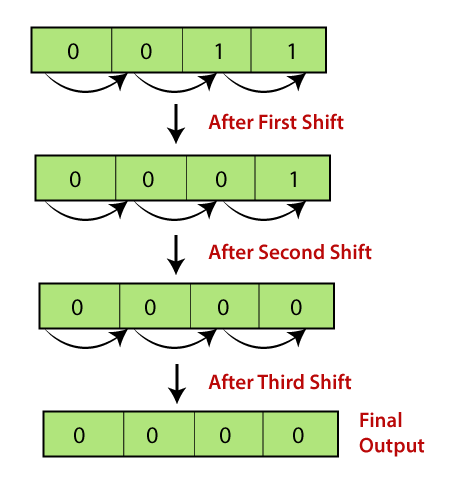
\includegraphics[scale=0.4]{bitwise}%
\caption{Bitwise shift}%
\label{}%
\end{figure}

In the above example, the value of 'x' is 3 and its binary value is 0011. We are shifting the value of 'x' by three-bit position to the right. Let's understand through the diagrammatic representation. Let's see a simple example.

\begin{lstlisting}
#include <iostream>  
using namespace std;  
int main()  
{  
	int x=5;   // variable declaration  
	std::cout << (x>>1) << std::endl;  
	return 0;  
}  
\end{lstlisting}

In the above code, we have declared a variable 'x'. After declaration, we applied the bitwise operator, i.e., right shift operator to shift one-bit position to right.

Output

\begin{verbatim}
2
\end{verbatim}

Let's look at another example.

\begin{lstlisting}
#include <iostream>  
using namespace std;  
int main()  
{  
 int x=7;   // variable declaration  
std::cout << (x<<3) << std::endl;  
return 0;  
}  
\end{lstlisting}

In the above code, we have declared a variable 'x'. After declaration, we applied the left shift operator to variable 'x' to shift the three-bit position to the left.

Output

\begin{Verbatim}
56
\end{Verbatim}

\subsubsection{Special Assignment Expressions}

Special assignment expressions are the expressions which can be further classified depending upon the value assigned to the variable. Few special assignment expressions are as follows. 

\begin{enumerate}
	\item Chained Assignment
	\item Embedded Assignment Expression
	\item Compound Assignment
\end{enumerate}

Chained assignment expression is an expression in which the same value is assigned to more than one variable by using single statement. For example:

\begin{lstlisting}
a=b=20   
 or   
(a=b) = 20  
\end{lstlisting}

Let's understand through an example.

\begin{lstlisting}
#include <iostream>  
using namespace std;  
int main()  
  
 int a;   // variable declaration  
 int b;   // variable declaration  
 a=b=80;  // chained assignment  
 std::cout <<"Values of 'a' and 'b' are : " <<a<<","<<b<< std::endl;  
 return 0;  
}  
\end{lstlisting}

In the above code, we have declared two variables, i.e., 'a' and 'b'. Then, we have assigned the same value to both the variables using chained assignment expression.

Output

\begin{Verbatim}
Values of 'a' and 'b' are : 80,80  
\end{Verbatim}

Note: Using chained assignment expression, the value cannot be assigned to the variable at the time of declaration. For example, int a=b=c=90 is an invalid statement.

\subsubsection{Embedded Assignment Expression}

An embedded assignment expression is an assignment expression in which assignment expression is enclosed within another assignment expression. Let's understand through an example.

\begin{lstlisting}
#include <iostream>  
using namespace std;  
int main()  
{  
 int a;  // variable declaration  
 int b;  // variable declaration  
 a=10+(b=90);  // embedded assignment expression  
 std::cout <<"Values of 'a' is " <<a<< std::endl;  
 return 0;  
}  
\end{lstlisting}

In the above code, we have declared two variables, i.e., 'a' and 'b'. Then, we applied embedded assignment expression (a=10+(b=90)).

Output

\begin{Verbatim}
Values of 'a' is 100  
\end{Verbatim}

\subsubsection{Compound Assignment}

A compound assignment expression is an expression which is a combination of an assignment operator and binary operator. 
For example,

\begin{Verbatim}
a+=10;   
\end{Verbatim}

In the above statement, 'a' is a variable and '+=' is a compound statement. Let's understand through an example.

\begin{lstlisting}
#include <iostream>  
using namespace std;  
int main()  
{  
  int a=10;   // variable declaration  
  a+=10;    // compound assignment  
  std::cout << "Value of a is :" <<a<< std::endl; // displaying the value of a.  
  return 0;  
}  
\end{lstlisting}

In the above code, we have declared a variable 'a' and assigns 10 value to this variable. Then, we applied compound assignment operator (+=) to 'a' variable, i.e., a+=10 which is equal to (a=a+10). This statement increments the value of 'a' by 10.

Output

\begin{Verbatim}
Value of a is :20 
\end{Verbatim} 

\chapter{Functional programming}

\section{Conditional statements}

In C++ programming, if statement is used to test the condition. There are various types of if statements in C++.

\begin{enumerate}
	\item if statement
\item if-else statement
\item nested if statement
\item if-else-if ladder
\end{enumerate}

\subsection{C++ IF Statement}

The C++ if statement tests the condition. It is executed if condition is true.

\begin{Verbatim}
if(condition){    
//code to be executed    
}  
\end{Verbatim}

%\begin{figure}%
%\centering 
%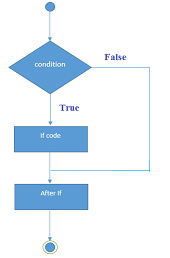
\includegraphics[width=\columnwidth]{cpp-if-else1}%
%\caption{}%
%\label{}%
%\end{figure}

C++ If Example

\begin{lstlisting}
#include <iostream>  
using namespace std;  
   
int main () {  
 int num = 10;    
	if (num % 2 == 0)    
	{    
		cout<<"It is even number";    
	}   
 return 0;  
}  
\end{lstlisting}

Output:

\begin{Verbatim}
It is even number
\end{Verbatim}

\subsection{C++ IF-else Statement}

The C++ if-else statement also tests the condition. It executes if block if condition is true otherwise else block is executed. The syntax for if-else is as follows. 

\begin{lstlisting}
if(condition){    
//code if condition is true    
}else{    
//code if condition is false    
}    
\end{lstlisting}

C++ If-else Example

\begin{lstlisting}
#include <iostream>  
using namespace std;  
int main () {  
   int num = 11;    
	if (num % 2 == 0)    
	{    
		cout<<"It is even number";    
	}   
	else  
	{    
		cout<<"It is odd number";    
	}  
   return 0;  
}  

\end{lstlisting}

Output:

\begin{Verbatim}
It is odd number
\end{Verbatim} 

\subsubsection{C++ If-else Example: with input from user}

\begin{lstlisting}
#include <iostream>  
using namespace std;  
int main () {  
	int num;  
	cout<<"Enter a Number: ";  
	cin>>num;  
	if (num % 2 == 0)    
	{    
		cout<<"It is even number"<<endl;    
	}   
	else  
	{    
		cout<<"It is odd number"<<endl;    
	}  
	return 0;  
}  
\end{lstlisting}

Output:

\begin{lstlisting}
Enter a number:11
It is odd number
\end{lstlisting}

Output:

\begin{lstlisting}
Enter a number:12
It is even number
\end{lstlisting}

\subsection{C++ IF-else-if ladder Statement}

The C++ if-else-if ladder statement executes one condition from multiple statements. Following is the syntax for if-else-if ladder in C++. 

\begin{lstlisting}
if(condition1){    
//code to be executed if condition1 is true    
}else if(condition2){    
//code to be executed if condition2 is true    
}    
else if(condition3){    
//code to be executed if condition3 is true    
}    
...    
else{    
//code to be executed if all the conditions are false    
}    
\end{lstlisting}

C++ If else-if Example

\begin{lstlisting}
#include <iostream>  
using namespace std;  
int main () {  
 int num;  
 cout<<"Enter a number to check grade:";    
 cin>>num;  
	if (num <0 || num >100)    
	{    
		cout<<"wrong number";    
	}    
	else if(num >= 0 && num < 50){    
		cout<<"Fail";    
	}    
	else if (num >= 50 && num < 60)    
	{    
		cout<<"D Grade";    
	}    
	else if (num >= 60 && num < 70)    
	{    
		cout<<"C Grade";    
	}    
	else if (num >= 70 && num < 80)    
	{    
		cout<<"B Grade";    
	}    
	else if (num >= 80 && num < 90)    
	{    
		cout<<"A Grade";    
	}    
	else if (num >= 90 && num <= 100)    
	{    
		cout<<"A+ Grade";  
	}    
    }    
\end{lstlisting}

Output:

\begin{lstlisting}
Enter a number to check grade:66
C Grade

Enter a number to check grade:-2
wrong number
\end{lstlisting}

\section{C++ Switch}

The C++ switch statement executes one statement from multiple conditions. It is like if-else-if ladder statement in C++.

\begin{lstlisting}
switch(expression){      
case value1:      
 //code to be executed;      
 break;    
case value2:      
 //code to be executed;      
 break;    
......      
      
default:       
 //code to be executed if all cases are not matched;      
 break;    
}    
\end{lstlisting}

C++ Switch Example

\begin{lstlisting}
#include <iostream>  
using namespace std;  
int main () {  
 int num;  
 cout<<"Enter a number to check grade:";    
 cin>>num;  
	 switch (num)    
	{    
		case 10: cout<<"It is 10"; break;    
		case 20: cout<<"It is 20"; break;    
		case 30: cout<<"It is 30"; break;    
		default: cout<<"Not 10, 20 or 30"; break;    
	}    
}    
\end{lstlisting}

Output:

\begin{lstlisting}
Enter a number:
10
It is 10

Enter a number:
55
Not 10, 20 or 30
\end{lstlisting}

\section{C++ For Loop}

The C++ for loop is used to iterate a part of the program several times. If the number of iteration is fixed, it is recommended to use for loop than while or do-while loops. The C++ for loop is same as C/C#. We can initialize variable, check condition and increment/decrement value. The syntax is as follows.

\begin{lstlisting}
for(initialization; condition; incr/decr){    
//code to be executed    
}    
\end{lstlisting}

C++ For Loop Example

\begin{lstlisting}
#include <iostream>  
using namespace std;  
int main() {  
 for(int i=1;i<=10;i++){      
		cout<<i <<"\n";      
	}       
}   
\end{lstlisting}

Output 

\begin{lstlisting}
1
2
3
4
5
6
7
8
9
10
\end{lstlisting}

\subsection{C++ Nested For Loop}

In C++, we can use for loop inside another for loop, it is known as nested for loop. The inner loop is executed fully when outer loop is executed one time. So if outer loop and inner loop are executed 4 times, inner loop will be executed 4 times for each outer loop i.e. total 16 times. Let's see a simple example of nested for loop in C++.

\begin{lstlisting}
#include <iostream>  
using namespace std;  
   
int main () {  
for(int i=1;i<=3;i++){      
	for(int j=1;j<=3;j++){      
		cout<<i<<" "<<j<<"\n";      
	}     
}  
} 
\end{lstlisting}

Output 

\begin{lstlisting}
1 1
1 2
1 3
2 1
2 2 
2 3
3 1
3 2
3 3
\end{lstlisting}

\subsection{C++ Infinite For Loop}

If we use double semicolon in for loop, it will be executed infinite times. Let's see a simple example of infinite for loop in C++.

\begin{lstlisting}
#include <iostream>  
using namespace std;  
   
int main () {  
for (; ;)    
{    
	cout<<"Infinitive For Loop";    
}    
}    
\end{lstlisting}

\section{C++ While loop}

In C++, while loop is used to iterate a part of the program several times. If the number of iteration is not fixed, it is recommended to use while loop than for loop.

\begin{lstlisting}
while(condition){    
//code to be executed    
}    
\end{lstlisting}

Let's see a simple example of while loop to print table of 1.

\begin{lstlisting}
#include <iostream>  
using namespace std;  
int main() {         
int i=1;      
while(i<=10)   
{      
	cout<<i <<"\n";    
	i++;  
}       
}  
\end{lstlisting}

Ouput 

\begin{lstlisting}
1
2
3
4
5
6
7
8
9
10
\end{lstlisting}

\subsection{C++ Nested While Loop Example}

In C++, we can use while loop inside another while loop, it is known as nested while loop. The nested while loop is executed fully when outer loop is executed once. Let's see a simple example of nested while loop in C++ programming language.

\begin{lstlisting}
#include <iostream>  
using namespace std;  
int main () {  
int i=1;      
while(i<=3)     
{    
	int j = 1;    
	while (j <= 3)    
	{      
		cout<<i<<" "<<j<<"\n";      
		j++;  
	}     
i++;  
}  
}    
\end{lstlisting}

Output:

\begin{lstlisting}
1 1
1 2
1 3
2 1
2 2 
2 3
3 1
3 2
3 3
\end{lstlisting}

\subsection{C++ Infinitive While Loop}

We can also create infinite while loop by passing true as the test condition.

\begin{lstlisting}
#include <iostream>  
using namespace std;  
int main () {  
while(true)  
{    
	cout<<"Infinitive While Loop";    
}    
}
\end{lstlisting}

\subsection{C++ Do-While Loop}

The C++ do-while loop is used to iterate a part of the program several times. If the number of iteration is not fixed and you must have to execute the loop at least once, it is recommended to use do-while loop. The C++ do-while loop is executed at least once because condition is checked after loop body.

\begin{lstlisting}
do{    
//code to be executed    
}while(condition);  
\end{lstlisting}

Let's see a simple example of C++ do-while loop to print the table of 1.

\begin{lstlisting}
#include <iostream>  
using namespace std;  
int main() {  
int i = 1;    
do{    
	cout<<i<<"\n";    
	i++;    
} while (i <= 10) ;    
}  
\end{lstlisting}

Output:

\begin{lstlisting}
1
2
3
4
5
6
7
8
9
10
\end{lstlisting}

\subsection{C++ Nested do-while Loop}

In C++, if you use do-while loop inside another do-while loop, it is known as nested do-while loop. The nested do-while loop is executed fully for each outer do-while loop. Let's see a simple example of nested do-while loop in C++.

\begin{lstlisting}
#include <iostream>  
using namespace std;  
int main() {  
int i = 1;    
do{    
	int j = 1;          
	do{    
		cout<<i<<"\n";        
		j++;    
	} while (j <= 3) ;    
	i++;    
} while (i <= 3) ;     
}  
\end{lstlisting}

Output:

\begin{lstlisting}
1 1
1 2
1 3
2 1
2 2 
2 3
3 1
3 2
3 3
\end{lstlisting}

\subsection{C++ Infinitive do-while Loop}

In C++, if you pass true in the do-while loop, it will be infinitive do-while loop.

\begin{lstlisting}
do{    
//code to be executed    
}while(true);  
\end{lstlisting}

C++ Infinitive do-while Loop Example

\begin{lstlisting}
#include <iostream>  
using namespace std;  
int main() {  
do{    
	cout<<"Infinitive do-while Loop";    
	} while(true);     
}  
\end{lstlisting}

\section{C++ Break \& Continue Statement}

The C++ break is used to break loop or switch statement. It breaks the current flow of the program at the given condition. In case of inner loop, it breaks only inner loop.

\begin{lstlisting}
jump-statement;      
break;  
\end{lstlisting}

Let's see a simple example of C++ break statement which is used inside the loop.

\begin{lstlisting}
#include <iostream>  
using namespace std;  
int main() {  
for (int i = 1; i <= 10; i++)    
	{    
		if (i == 5)    
		{    
			break;    
		}    
	cout<<i<<"\n";    
	}    
}  
\end{lstlisting}

Output:

\begin{lstlisting}
1
2
3
4
\end{lstlisting}

\subsection{C++ Break Statement with Inner Loop}

The C++ break statement breaks inner loop only if you use break statement inside the inner loop. Let's see the example code:

\begin{lstlisting}
#include <iostream>  
using namespace std;  
int main()  
{  
for(int i=1;i<=3;i++){        
	for(int j=1;j<=3;j++){        
		if(i==2&&j==2){        
			break;        
		}        
			cout<<i<<" "<<j<<"\n";             
	}        
}    
} 
\end{lstlisting}
 
Output:

\begin{lstlisting}
1 1
1 2
1 3
2 1
3 1
3 2
3 3
\end{lstlisting}

\subsection{C++ Continue Statement}

The C++ continue statement is used to continue loop. It continues the current flow of the program and skips the remaining code at specified condition. In case of inner loop, it continues only inner loop.

\begin{lstlisting}
jump-statement;      
continue;     
\end{lstlisting}

C++ Continue Statement Example

\begin{lstlisting}
#include <iostream>  
using namespace std;  
int main()  
{  
 for(int i=1;i<=10;i++){      
	if(i==5){      
		continue;      
	}      
	cout<<i<<"\n";      
 }        
}  
\end{lstlisting}

Output:

\begin{lstlisting}
1
2
3
4
6
7
8
9
10
\end{lstlisting}

\subsection{C++ Continue Statement with Inner Loop}

C++ Continue Statement continues inner loop only if you use continue statement inside the inner loop.

\begin{lstlisting}
#include <iostream>  
using namespace std;  
int main()  
{  
 for(int i=1;i<=3;i++){        
	for(int j=1;j<=3;j++){        
	 if(i==2&&j==2){        
		continue;        
	 }        
	cout<<i<<" "<<j<<"\n";                  
	}        
 }            
}  
\end{lstlisting}

Output:

\begin{lstlisting}
1 1
1 2
1 3
2 1
2 3
3 1
3 2
3 3
\end{lstlisting}

\subsection{C++ Goto Statement}

The C++ goto statement is also known as jump statement. It is used to transfer control to the other part of the program. It unconditionally jumps to the specified label. It can be used to transfer control from deeply nested loop or switch case label. Let's see the simple example of goto statement in C++.

\begin{lstlisting}
#include <iostream>  
using namespace std;  
int main()  
{  
ineligible:    
  cout<<"You are not eligible to vote!\n";    
	cout<<"Enter your age:\n";    
	int age;  
	cin>>age;  
	if (age < 18){    
		goto ineligible;    
	}    
	else    
	{    
		cout<<"You are eligible to vote!";     
	}         
}  
\end{lstlisting}

Output:

\begin{lstlisting}
You are not eligible to vote!
Enter your age:
16
You are not eligible to vote!
Enter your age:
7
You are not eligible to vote!
Enter your age:
22
You are eligible to vote!
\end{lstlisting}

\section{Arrays}

Like other programming languages, array in C++ is a group of similar types of elements that have contiguous memory location. In C++ \texttt{std::array} is a container that encapsulates fixed size arrays. In C++, array index starts from 0. We can store only fixed set of elements in C++ array.

\begin{figure}[h]
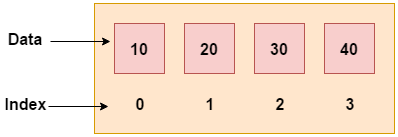
\includegraphics[width=\columnwidth]{c-array}%
\caption{Arrays in C++}%
\label{}%
\end{figure}

\subsection{Advantages of C++ Array}

\begin{enumerate}
	\item Code Optimization (less code)
\item Random Access
\item Easy to traverse data
\item Easy to manipulate data
\item Easy to sort data etc.

\end{enumerate}

However, there one potential disadvantage of an array is that they are \textsl{fixed size data structures}. 

\subsection{C++ Array Types}

There are 2 types of arrays in C++ programming:

\begin{enumerate}
	\item One Dimensional Array
\item Multidimensional Array
\end{enumerate}

\subsection{One Dimensional Array}

Let's see a simple example of C++ array, where we are going to create, initialize and traverse array.

\begin{lstlisting}
#include <iostream>  
using namespace std;  
int main()  
{  
 int arr[5]={10, 0, 20, 0, 30};  //creating and initializing array    
	//traversing array    
	for (int i = 0; i < 5; i++)    
	{    
		cout<<arr[i]<<"\n";    
	}    
}  
\end{lstlisting}


\section{Multidimensional arrays}

The multidimensional array is also known as rectangular arrays in C++. It can be two dimensional or three dimensional. The data is stored in tabular form (row ∗ column) which is also known as matrix. Let's see a simple example of multidimensional array in C++ which declares, initializes and traverse two dimensional arrays.

\begin{lstlisting}
#include <iostream>  
using namespace std;  
int main()  
{  
  int test[3][3];  //declaration of 2D array
	test[0][0]=5;  //initialization
	test[0][1]=10;   
	test[1][1]=15;  
	test[1][2]=20;  
	test[2][0]=30;  
	test[2][2]=10;  
	//traversal    
	for(int i = 0; i < 3; ++i)  
	{  
	for(int j = 0; j < 3; ++j)  
	{  
		cout<< test[i][j]<<" ";  
	}  
	cout<<"\n"; //new line at each row   
	}  
	return 0;  
}
\end{lstlisting}
  
Output:

\begin{lstlisting}
5 10 0 
0 15 20 
30 0 10 
\end{lstlisting}

\subsubsection{Declaration and initialization at same time}

Let's see a simple example of multidimensional array which initializes array at the time of declaration.

\begin{lstlisting}
#include <iostream>  
using namespace std;  
int main()  
{  
int test[3][3] =  
{  
	{2, 5, 5},  
	{4, 0, 3},  
	{9, 1, 8}  };  //declaration and initialization    
//traversal    
for(int i = 0; i < 3; ++i)  
{  
	for(int j = 0; j < 3; ++j)  
	{  
			cout<< test[i][j]<<" ";  
	}  
	cout<<"\n"; //new line at each row   
}  
return 0;  
}  
\end{lstlisting}

\section{Functions in C/C++}

A function is a set of statements that take inputs, do some specific computation and produces output. The idea is to put some commonly or repeatedly done task together and make a function so that instead of writing the same code again and again for different inputs, we can call the function.

The general form of a function is:

\begin{lstlisting}
return_type function_name([ arg1_type arg1_name, ... ]) { code }
\end{lstlisting}

Example:

Below is a simple C/C++ program to demonstrate functions.

\begin{lstlisting}
#include <iostream>
using namespace std;
  
int max(int x, int y) 
{ 
	if (x > y) 
	return x; 
	else
	return y; 
} 
  
int main() {
	int a = 10, b = 20; 

	// Calling above function to find max of 'a' and 'b' 
	int m = max(a, b); 

	cout << "m is " << m; 
	return 0; 
} 
\end{lstlisting}

Output:

\begin{verbatim}
m is 20
\end{verbatim}

\subsection{Why do we need functions?}

\begin{enumerate}
	\item Functions help us in reducing code redundancy. If functionality is performed at multiple places in software, then rather than writing the same code, again and again, we create a function and call it everywhere. This also helps in maintenance as we have to change at one place if we make future changes to the functionality.
\item Functions make code modular. Consider a big file having many lines of code. It becomes really simple to read and use the code if the code is divided into functions.
\item Functions provide abstraction. For example, we can use library functions without worrying about their internal working.
\end{enumerate}

\subsection{Function Declaration}

A function declaration tells the compiler about the number of parameters function takes, data-types of parameters, and return type of function. Putting parameter names in function declaration is optional in the function declaration, but it is necessary to put them in the definition. Below are an example of function declarations. 

\begin{lstlisting}
// A function that takes two integers as parameters
// and returns an integer
int max(int, int);

// A function that takes an int pointer and an int variable as parameters
// and returns a pointer of type int
int *swap(int*,int);

// A function that takes a charas parameters
// and returns an reference variable
char *call(char b);

// A function that takes a char and an int as parameters
// and returns an integer
int fun(char, int);

\end{lstlisting}

\subsection{Return From Void Functions}

Void functions are known as Non-Value Returning functions. They are \enquote{void} due to the fact that they are not supposed to return values. We cannot return values but there is something we can surely return from void functions. Void functions do not have a return type, but they can do return values. Some of the cases are listed below:

\begin{enumerate}
	\item  \textit{A Void Function Can Return}: We can simply write a return statement in a void fun(). In fact, it is considered a good practice (for readability of code) to write a return; statement to indicate the end of the function. 
	
	\begin{lstlisting}
// CPP Program to demonstrate void functions
#include <iostream>
using namespace std;
  
void fun()
{
	cout << "Hello";

	// We can write return in void
	return;
}
  
// Driver Code
int main()
{
	fun();
	return 0;
}
	\end{lstlisting}

\item \textit{A void \textit{fun()} can return another void function}: A void function can also call another void function while it is terminating. For example, 

	\begin{lstlisting}
// C++ code to demonstrate void()
// returning void()
#include <iostream>
using namespace std;
  
// A sample void function
void work()
{
	cout << "The void function has returned "
					" a void() !!! \n";
}
  
// Driver void() returning void work()
void test()
{
	// Returning void function
	return work();
}
  
// Driver Code
int main()
{
	// Calling void function
	test();
	return 0;
}
\end{lstlisting}

\item \textit{A \textit{void()} can return a void value}: A \textit{void()} cannot return a value that can be used. But it can return a value that is void without giving an error. For example,

	\begin{lstlisting}
// C++ code to demonstrate void()
// returning a void value
#include <iostream>
using namespace std;
  
// Driver void() returning a void value
void test()
{
	cout << "Hello";

	// Returning a void value
	return (void)"Doesn't Print";
}
  
// Driver Code
int main()
{
	test();
	return 0;
}
	\end{lstlisting}
\end{enumerate}

\subsection{Parameter Passing to functions}

The parameters passed to function are called \textit{actual parameters}. For example, in the above program 10 and 20 are actual parameters. The parameters received by function are called \textit{formal parameters}. For example, in the above program x and y are formal parameters. There are two most popular ways to pass parameters.

\begin{enumerate}
	\item Pass by Value: In this parameter passing method, values of actual parameters are copied to function’s formal parameters and the two types of parameters are stored in different memory locations. So any changes made inside functions are not reflected in actual parameters of caller.
\item Pass by Reference Both actual and formal parameters refer to same locations, so any changes made inside the function are actually reflected in actual parameters of caller.

\end{enumerate}

Parameters are always passed by value in C. For example. in the below code, value of x is not modified using the function \textit{fun()}.

\begin{lstlisting}
#include <iostream>
using namespace std;

void fun(int x) {
	x = 30;
}

int main() {
	int x = 20;
	fun(x);
	cout << "x = " << x;
	return 0;
}

\end{lstlisting}

Output:

\begin{lstlisting}
x = 20
\end{lstlisting}

However, in C, we can use pointers to get the effect of pass-by reference. For example, consider the below program. The function \textit{fun()} expects a pointer ptr to an integer (or an address of an integer). It modifies the value at the address ptr. The dereference operator * is used to access the value at an address. In the statement \enquote{*ptr = 30}, value at address \textit{ptr} is changed to 30. The address operator $\&$ is used to get the address of a variable of any data type. In the function call statement \enquote{fun(\&x)}, the address of x is passed so that x can be modified using its address.

\begin{lstlisting}
#include <iostream>
using namespace std;

void fun(int *ptr)
{
	*ptr = 30;
}

int main() {
	int x = 20;
	fun(&x);
	cout << "x = " << x;
	
	return 0;
}

\end{lstlisting}

Output:

\begin{verbatim}
x = 30
\end{verbatim}


\section{Pointers}

Pointers are symbolic representation of addresses. They enable programs to simulate call-by-reference as well as to create and manipulate dynamic data structures. The pointer in C++ language is a variable, it is also known as locator or indicator that points to an address of a value.

\begin{figure}[h]
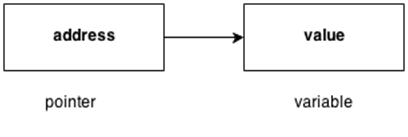
\includegraphics[width=\columnwidth]{pointers}%
\caption{Pointers}%
\label{}%
\end{figure}

\subsection{Advantage of pointer}

\begin{enumerate}
	\item Pointer reduces the code and improves the performance, it is used to retrieving strings, trees etc. and used with arrays, structures and functions.

\item We can return multiple values from function using pointer.
\item It makes you able to access any memory location in the computer's memory.
\item  \textit{Dynamic memory allocation}: We can dynamically allocate memory using \texttt{malloc()} and \texttt{calloc()} functions where pointer is used.
	\item \textit{Arrays, Functions and Structures}: Pointers in c language are widely used in arrays, functions and structures. It reduces the code and improves the performance.
\end{enumerate}

\subsection{Usage of pointer}

There are many usage of pointers in C++ language.

\begin{enumerate}
\item Define a pointer variable
\item Assigning the address of a variable to a pointer using unary operator (&) which returns the address of that variable.
\item Accessing the value stored in the address using unary operator (*) which returns the value of the variable located at the address specified by its operand.
		
\end{enumerate}

\begin{figure}[h]
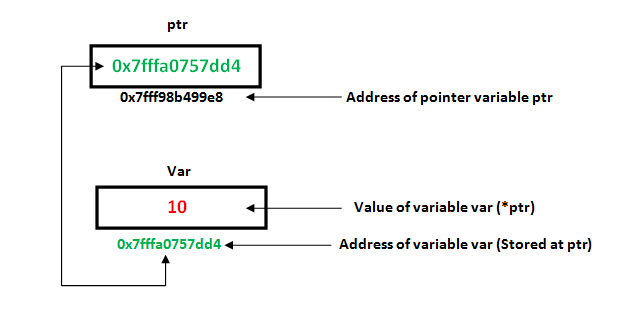
\includegraphics[width=\columnwidth]{pointers-in-c}
\caption{Declaring pointers}%
\label{}%
\end{figure}


\subsection{Symbols used in pointer}

\begin{table}[h]
\centering 
\begin{tabular}{lll} \hline 
Symbol	& Name	& Description \\ \hline 
\& (ampersand sign)	& Address & Determine \\ 
& operator	& the address \\
& &  of a variable. \\
* (asterisk sign)	& Indirection & Access \\ 
& operator	& the value \\
& & of an address. \\ \hline 
\end{tabular}
\caption{Symbols used for pointers}
\label{}
\end{table}

\subsection{Declaring a pointer}

The pointer in C++ language can be declared using ∗ (asterisk symbol).

\begin{verbatim}
int *   a; //pointer to int    
char *  c; //pointer to char    
\end{verbatim}

\subsection{Pointer Example}

Let's see the simple example of using pointers printing the address and value.

\begin{lstlisting}
#include <iostream>  
using namespace std;  
int main()  {  
	int number=30;    
	int *   p;      
	p=&number;//stores the address of number variable    
	cout<<"Address of number variable is:"<<&number<<endl;    
	cout<<"Address of p variable is:"<<p<<endl;    
	cout<<"Value of p variable is:"<<*p<<endl;    
  return 0;  
}  
\end{lstlisting}

Output:

\begin{verbatim}
Address of number variable is:0x7ffccc8724c4
Address of p variable is:0x7ffccc8724c4
Value of p variable is:30  

\end{verbatim}

The other example using functions 

\begin{lstlisting}
// C++ program to illustrate Pointers in C++
  
#include <bits/stdc++.h>
using namespace std;
void pointer_test()
{
	int var = 20; 
		
			//declare pointer variable    
	int *ptr; 
		
	//note that data type of ptr and var must be same
	ptr = &var;    

	// assign the address of a variable to a pointer
	cout << "Value at ptr = " << ptr << "\n";
	cout << "Value at var = " << var << "\n";
	cout << "Value at *ptr = " << *ptr << "\n";     
}
//Driver program
int main()
{
	pointer_test();
}
\end{lstlisting}

Output 

\begin{verbatim}
Value at ptr = 0x7ffcb9e9ea4c
Value at var = 20
Value at *ptr = 20
\end{verbatim}

\subsection{Pointer Expressions and Pointer Arithmetic}

A limited set of arithmetic operations can be performed on pointers which are:

\begin{enumerate}
	\item incremented ( ++ )
\item decremented ( — )
\item an integer may be added to a pointer ( + or += )
\item an integer may be subtracted from a pointer ( – or -= )
\item difference between two pointers (p1-p2)

\end{enumerate}

Pointer arithmetic on arrays using loops

\begin{lstlisting}
// C++ program to illustrate Pointer Arithmetic in C++
#include <bits/stdc++.h>
using namespace std;
void pointer_in_loops() {
	//Declare an array
	int v[3] = {10, 100, 200};
		
	//declare pointer variable 
	int *ptr;
		
	//Assign the address of v[0] to ptr
	ptr = v;
		
	for (int i = 0; i < 3; i++) {
		cout << "Value at ptr = " << ptr << "\n";
		cout << "Value at *ptr = " << *ptr << "\n";
			
		// Increment pointer ptr by 1 
		ptr++;
	}
}
  
//Driver program
int main()
{
	pointer_in_loops();
}
\end{lstlisting}

Output 

\begin{verbatim}
Output:
Value at ptr = 0x7fff9a9e7920
Value at *ptr = 10
Value at ptr = 0x7fff9a9e7924
Value at *ptr = 100
Value at ptr = 0x7fff9a9e7928
Value at *ptr = 200
\end{verbatim}


\begin{comment} 

Pointer Program to swap 2 numbers without using 3rd variable

\begin{lstlisting}
#include <iostream>  
using namespace std;  
int main()  {  
	int a=20,b=10,*p1=&a,*p2=&b;    
	cout<<"Before swap: *p1="<<*p1<<" *p2="<<*p2<<endl;    
	*p1=*p1+*p2;    
	*p2=*p1-*p2;    
	*p1=*p1-*p2;    
	cout<<"After swap: *p1="<<*p1<<" *p2="<<*p2<<endl;    
  return 0;  
}  
\end{lstlisting}
\end{comment} 

\subsection{References and Pointers}

There are 3 ways to pass C++ arguments to a function:

\begin{enumerate}
	\item call-by-value
\item call-by-reference with pointer argument
\item call-by-reference with reference argument
\end{enumerate}

\begin{lstlisting}
// C++ program to illustrate call-by-methods in C++

#include <bits/stdc++.h>
using namespace std;
//Pass-by-Value
int square1(int n)
{
	//Address of n in square1() is not the same as n1 in main()
	cout << "address of n1 in square1(): " << &n << "\n";
	
	// clone modified inside the function
	n *= n;
	return n;
}
//Pass-by-Reference with Pointer Arguments
void square2(int *n)
{
	//Address of n in square2() is the same as n2 in main()
	cout << "address of n2 in square2(): " << n << "\n";
	
	// Explicit de-referencing to get the value pointed-to
	*n *= *n;
}
//Pass-by-Reference with Reference Arguments
void square3(int &n)
{
	//Address of n in square3() is the same as n3 in main()
	cout << "address of n3 in square3(): " << &n << "\n";
	
	// Implicit de-referencing (without '*')
	n *= n;
}
void Main()
{
	//Call-by-Value
	int n1=8;
	cout << "address of n1 in main(): " << &n1 << "\n";
	cout << "Square of n1: " << square1(n1) << "\n";
	cout << "No change in n1: " << n1 << "\n";
	
	//Call-by-Reference with Pointer Arguments
	int n2=8;
	cout << "address of n2 in main(): " << &n2 << "\n";
	square2(&n2);
	cout << "Square of n2: " << n2 << "\n";
	cout << "Change reflected in n2: " << n2 << "\n";
	
	//Call-by-Reference with Reference Arguments
	int n3=8;
	cout << "address of n3 in main(): " << &n3 << "\n";
	square3(n3);
	cout << "Square of n3: " << n3 << "\n";
	cout << "Change reflected in n3: " << n3 << "\n";
	
	
}
//Driver program
int main()
{
	Main();
}
\end{lstlisting}


Output 

\begin{lstlisting}
address of n1 in main(): 0x7ffcdb2b4a44
address of n1 in square1(): 0x7ffcdb2b4a2c
Square of n1: 64
No change in n1: 8
address of n2 in main(): 0x7ffcdb2b4a48
address of n2 in square2(): 0x7ffcdb2b4a48
Square of n2: 64
Change reflected in n2: 64
address of n3 in main(): 0x7ffcdb2b4a4c
address of n3 in square3(): 0x7ffcdb2b4a4c
Square of n3: 64
Change reflected in n3: 64
\end{lstlisting}

\chapter{C++ OOPs Concepts}

The major purpose of C++ programming is to introduce the concept of object orientation to the C programming language. Object Oriented Programming is a paradigm that provides many concepts such as inheritance, data binding, polymorphism etc. The programming paradigm where everything is represented as an object is known as truly object-oriented programming language. 

\subsection{OOPs (Object Oriented Programming System)}

Object means a real word entity such as pen, chair, table etc. Object-Oriented Programming is a methodology or paradigm to design a program using classes and objects. It simplifies the software development and maintenance by providing some concepts:

\begin{enumerate}
	\item Object
\item Class
\item Inheritance
\item Polymorphism
\item Abstraction
\item Encapsulation
\end{enumerate}

\subsubsection{Object}
Any entity that has state and behavior is known as an object. For example: chair, pen, table, keyboard, bike etc. It can be physical and logical.

\subsubsection{Class}
Collection of objects is called class. It is a logical entity.

\subsubsection{Inheritance}
When one object acquires all the properties and behaviours of parent object i.e. known as inheritance. It provides code reusability. It is used to achieve runtime polymorphism.

\subsubsection{Polymorphism}
When one task is performed by different ways i.e. known as polymorphism. For example: to convince the customer differently, to draw something e.g. shape or rectangle etc. In C++, we use Function overloading and Function overriding to achieve polymorphism.

\subsubsection{Abstraction}
Hiding internal details and showing functionality is known as abstraction. For example: phone call, we don't know the internal processing. In C++, we use abstract class and interface to achieve abstraction.

\subsubsection{Encapsulation}
Binding (or wrapping) code and data together into a single unit is known as encapsulation. For example: capsule, it is wrapped with different medicines.


\subsection{Advantage of OOPs over Procedure-oriented programming language}
\begin{enumerate}
	\item OOPs makes development and maintenance easier where as in Procedure-oriented programming language it is not easy to manage if code grows as project size grows.
	\item OOPs provide data hiding whereas in Procedure-oriented programming language a global data can be accessed from anywhere.
\item OOPs provide ability to simulate real-world event much more effectively. We can provide the solution of real word problem if we are using the Object-Oriented Programming language.

\end{enumerate}

\section{C++ Object and Class}

Since C++ is an object-oriented language, program is designed using objects and classes in C++. In C++, Object is a real world entity, for example, chair, car, pen, mobile, laptop etc. In other words, object is an entity that has state and behavior. Here, state means data and behavior means functionality. Object is a runtime entity, it is created at runtime. Object is an instance of a class. All the members of the class can be accessed through object. Let's see an example to create object of student class using s1 as the reference variable.

\begin{verbatim}
Student s1;  //creating an object of Student   
\end{verbatim}

In this example, Student is the type and s1 is the reference variable that refers to the instance of Student class.

\subsection{C++ Class}
In C++, class is a group of similar objects. It is a template from which objects are created. It can have fields, methods, constructors etc. Let's see an example of C++ class that has three fields only.

\begin{lstlisting}
class Student    
 {    
     public:  
     int id;  //field or data member     
     float salary; //field or data member  
     String name;//field or data member    
 }    
\end{lstlisting} 

\subsubsection{C++ Object and Class Example}
Let's see an example of class that has two fields: \textit{id }and \textit{name}. It creates instance of the class, initializes the object and prints the object value.

\begin{lstlisting}
#include <iostream>  
using namespace std;  
class Student {  
   public:  
      int id;//data member (also instance variable)      
      string name;//data member(also instance variable)      
};  
int main() {  
    Student s1; //creating an object of Student   
    s1.id = 201;    
    s1.name = "Sonoo Jaiswal";   
    cout<<s1.id<<endl;  
    cout<<s1.name<<endl;  
    return 0;  
}  
\end{lstlisting} 

Output:

\begin{verbatim}
201
Sonoo Jaiswal
\end{verbatim}

\subsection{C++ Class Example: Initialize and Display data through method}

Let's see another example of C++ class where we are initializing and displaying object through method.

\begin{lstlisting}
#include <iostream>  
using namespace std;  
class Student {  
   public:  
       int id;//data member (also instance variable)      
       string name;//data member(also instance variable)      
       void insert(int i, string n)    
        {    
            id = i;    
            name = n;    
        }    
       void display()    
        {    
            cout<<id<<"  "<<name<<endl;    
        }    
};  
int main(void) {  
    Student s1; //creating an object of Student   
    Student s2; //creating an object of Student  
    s1.insert(201, "Sonoo");    
    s2.insert(202, "Nakul");    
    s1.display();    
    s2.display();  
    return 0;  
}  
\end{lstlisting} 

Output:

\begin{verbatim}
201  Sonoo
202  Nakul
\end{verbatim}

\subsection{C++ Class Example: Store and Display Employee Information}

Let's see another example of C++ class where we are storing and displaying employee information using method.

\begin{lstlisting}
#include <iostream>  
using namespace std;  
class Employee {  
   public:  
       int id;//data member (also instance variable)      
       string name;//data member(also instance variable)  
       float salary;  
       void insert(int i, string n, float s)    
        {    
            id = i;    
            name = n;    
            salary = s;  
        }    
       void display()    
        {    
            cout<<id<<"  "<<name<<"  "<<salary<<endl;    
        }    
};  
int main(void) {  
    Employee e1; //creating an object of Employee   
    Employee e2; //creating an object of Employee  
    e1.insert(201, "Sonoo",990000);    
    e2.insert(202, "Nakul", 29000);    
    e1.display();    
    e2.display();    
    return 0;  
}  
\end{lstlisting} 

Output:

\begin{verbatim}
201  Sonoo  990000
202  Nakul  29000
\end{verbatim}

\section{C++ Constructor}

In C++, constructor is a special method which is invoked automatically at the time of object creation. It is used to initialize the data members of new object generally. The constructor in C++ has the same name as class or structure. There can be two types of constructors in C++.

\begin{enumerate}
	\item Default constructor
\item Parameterized constructor

\end{enumerate}

\subsection{C++ Default Constructor}

A constructor which has no argument is known as default constructor. It is invoked at the time of creating object. Let's see the simple example of C++ default Constructor.

\begin{lstlisting}
#include <iostream>  
using namespace std;  
class Employee  
 {  
   public:  
		Employee()    
		{    
			cout<<"Default Constructor Invoked"<<endl;    
		}    
};  
int main(void)   
{  
	Employee e1; //creating an object of Employee   
	Employee e2;   
	return 0;  
}  
\end{lstlisting}

Output:

\begin{verbatim}
Default Constructor Invoked 
Default Constructor Invoked
\end{verbatim}

\subsection{C++ Parameterized Constructor}

A constructor which has parameters is called parameterized constructor. It is used to provide different values to distinct objects. Let's see the simple example of C++ Parameterized Constructor.

\begin{lstlisting}
#include <iostream>
using namespace std;
class Employee {
 public:
	 int id;//data member (also instance variable)    
	 string name;//data member(also instance variable)
	 float salary;
	 Employee(int i, string n, float s)  
		{  
				id = i;  
				name = n;  
				salary = s;
		}  
	 void display()  
		{  
				cout<<id<<"  "<<name<<"  "<<salary<<endl;  
		}  
};
int main(void) {
	Employee e1 =Employee(101, "Sonoo", 890000); //creating an object of Employee 
	Employee e2=Employee(102, "Nakul", 59000); 
	e1.display();  
	e2.display();  
	return 0;
}
\end{lstlisting} 

Output:

\begin{verbatim}
101  Sonoo  890000
102  Nakul  59000
\end{verbatim} 

\section{C++ Destructor}

A destructor works opposite to constructor; it destructs the objects of classes. It can be defined only once in a class. Like constructors, it is invoked automatically. 
A destructor is defined like constructor. It must have same name as class. But it is prefixed with a tilde sign $(~)$.

\subsubsection{C++ Constructor and Destructor Example}

Let's see an example of constructor and destructor in C++ which is called automatically.

\begin{lstlisting}
#include <iostream>  
using namespace std;  
class Employee  
 {  
   public:  
		Employee()    
		{    
			cout<<"Constructor Invoked"<<endl;    
		}    
		~Employee()    
		{    
			cout<<"Destructor Invoked"<<endl;    
		}  
};  
int main(void)   
{  
	Employee e1; //creating an object of Employee   
	Employee e2; //creating an object of Employee  
	return 0;  
}
\end{lstlisting}
  
Output:

\begin{verbatim} 
Constructor Invoked
Constructor Invoked
Destructor Invoked
Destructor Invoked
\end{verbatim} 

\subsubsection{Destructor example: string operations}

\begin{lstlisting}
class String {
private:
	char* s;
	int size;
 
public:
	String(char*); // constructor
	~String(); // destructor
};
 
String::String(char* c)
{
	size = strlen(c);
	s = new char[size + 1];
	strcpy(s, c);
}
String::~String() { delete[] s; }
\end{lstlisting} 

% https://www.algbly.com/Tutorials/Cpp-programming/Cpp-destructor.html [more on destructors]

\section{C++ this Pointer}

In C++ programming, \textbf{this} is a keyword that refers to the current instance of the class. There can be 3 main usage of \textit{this} keyword in C++.

\begin{enumerate}
	\item It can be used to pass current object as a parameter to another method.
\item It can be used to refer current class instance variable.
\item It can be used to declare indexers.
\end{enumerate}

\subsubsection{C++ this Pointer Example}

Let's see the example of this keyword in C++ that refers to the fields of current class.

\begin{lstlisting} 
#include <iostream>  
using namespace std;  
class Employee {  
 public:  
	 int id; //data member (also instance variable)      
	 string name; //data member(also instance variable)  
	 float salary;  
	 Employee(int id, string name, float salary)    
		{    
			this->id = id;    
			this->name = name;    
			this->salary = salary;   
		}    
	 void display()    
		{    
			cout<<id<<"  "<<name<<"  "<<salary<<endl;    
		}    
};  
int main(void) {  
    Employee e1 =Employee(101, "Sonoo", 890000); //creating an object of Employee   
    Employee e2=Employee(102, "Nakul", 59000); //creating an object of Employee  
    e1.display();    
    e2.display();    
    return 0;  
}  
\end{lstlisting} 

Output:

\begin{verbatim}
101  Sonoo  890000
102  Nakul  59000
\end{verbatim}

\section{C++ static}

In C++, \texttt{static} is a keyword or modifier that belongs to the type not instance. So instance is not required to access the static members. In C++, static can be field, method, constructor, class, properties, operator and event.\textbf{\textit{ static} keyword is used to achieve memory efficiency in programming}. 

\subsection{C++ Static Field}

A field which is declared as static is called static field. Unlike instance field which gets memory each time whenever you create object, there is only one copy of static field created in the memory. It is shared to all the objects. It is used to refer the common property of all objects such as rateOfInterest in case of Account, companyName in case of Employee etc.

Let's see the simple example of static field in C++.

\begin{lstlisting}
#include <iostream>  
using namespace std;  
class Account {  
 public:  
	 int accno; //data member (also instance variable)      
	 string name; //data member(also instance variable)  
	 static float rateOfInterest;   
	 Account(int accno, string name)   
		{    
			this->accno = accno;    
			this->name = name;    
		}    
	 void display()    
		{    
			cout<<accno<< "<<name<< " "<<rateOfInterest<<endl;   
		}    
};  
float Account::rateOfInterest=6.5;  
int main(void) {  
    Account a1 =Account(201, "Sanjay"); //creating an object of Employee   
    Account a2=Account(202, "Nakul"); //creating an object of Employee  
    a1.display();    
    a2.display();    
    return 0;  
}  
\end{lstlisting} 

Output:

\begin{verbatim}
201 Sanjay 6.5
202 Nakul 6.5
\end{verbatim}

Let's see another example of static keyword in C++ which counts the objects.

\begin{lstlisting}
#include <iostream>  
using namespace std;  
class Account {  
 public:  
	 int accno; //data member (also instance variable)      
	 string name;   
	 static int count;     
	 Account(int accno, string name)   
		{    
		  this->accno = accno;    
			this->name = name;    
			count++;  
		}    
	 void display()    
		{    
			cout<<accno<<" "<<name<<endl;   
		}    
};  
int Account::count=0;  
int main(void) {  
	Account a1 =Account(201, "Sanjay"); //creating an object of Account  
	Account a2=Account(202, "Nakul");   
	 Account a3=Account(203, "Ranjana");  
	a1.display();    
	a2.display();    
	a3.display();    
	cout<<"Total Objects are: "<<Account::count;  
	return 0;  
}  
\end{lstlisting} 

Output:

\begin{verbatim}
201 Sanjay
202 Nakul
203 Ranjana
Total Objects are: 3
\end{verbatim} 

\section{C++ Inheritance}

In C++, inheritance is a process in which one object acquires all the properties and behaviors of its parent object automatically. In such way, you can reuse, extend or modify the attributes and behaviors which are defined in other class.

In C++, the class which inherits the members of another class is called derived class and the class whose members are inherited is called base class. The derived class is the specialized class for the base class. Main purpose of inheritance is \textit{Code reusability}. 

\subsection{Types Of Inheritance}

C++ supports five types of inheritance:

\begin{enumerate}
	\item Single inheritance
\item Multiple inheritance
\item Hierarchical inheritance
\item Multilevel inheritance
\item Hybrid inheritance
\end{enumerate}

\begin{figure}%
\centering
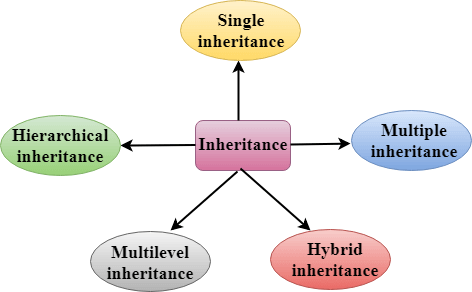
\includegraphics[width=\columnwidth]{cpp-inheritance}%
\caption{Types of inheritance in C++}%
\label{}%
\end{figure}

\subsubsection{Derived Classes}

A Derived class is defined as the class derived from the base class.

The Syntax of Derived class:

\begin{lstlisting} 
class derived_class_name :: visibility-mode base_class_name  
{  
    // body of the derived class.  
}  
\end{lstlisting}

Where,

\textit{derived\_class\_name}: It is the name of the derived class.

\textit{visibility mode}: The visibility mode specifies whether the features of the base class are publicly inherited or privately inherited. It can be public or private.

\textit{base\_class\_name}: It is the name of the base class.

When the base class is privately inherited by the derived class, public members of the base class becomes the private members of the derived class. Therefore, the public members of the base class are not accessible by the objects of the derived class only by the member functions of the derived class.

When the base class is publicly inherited by the derived class, public members of the base class also become the public members of the derived class. Therefore, the public members of the base class are accessible by the objects of the derived class as well as by the member functions of the base class. In C++, the default mode of visibility is private. \textit{\textbf{The private members of the base class are never inherited.}}

\subsection{C++ Single Inheritance}

Single inheritance is defined as the inheritance in which a derived class is inherited from the only one base class. 

\begin{figure}[h]

\includegraphics[width=\columnwidth]{single-inheritance}%
\caption{Single inheritance}%
\label{}%
\end{figure}

Where 'A' is the base class, and 'B' is the derived class.

\subsubsection{C++ Single Level Inheritance Example: Inheriting Fields}

When one class inherits another class, it is known as single level inheritance. Let's see the example of single level inheritance which inherits the fields only.

\begin{lstlisting} 
#include <iostream>  
using namespace std;  
 class Account {  
   public:  
   float salary = 60000;   
 };  
   class Programmer: public Account {  
   public:  
   float bonus = 5000;    
   };       
int main(void) {  
	 Programmer p1;  
	 cout<<"Salary: "<<p1.salary<<endl;    
	 cout<<"Bonus: "<<p1.bonus<<endl;    
	return 0;  
}  
\end{lstlisting} 

Output:

\begin{verbatim}
Salary: 60000
Bonus: 5000

\end{verbatim}

In the above example, Employee is the base class and Programmer is the derived class.

\subsubsection{C++ Single Level Inheritance Example: Inheriting Methods}

Let's see another example of inheritance in C++ which inherits methods only.

\begin{lstlisting}
#include <iostream>  
using namespace std;  
 class Animal {  
   public:  
 void eat() {   
    cout<<"Eating..."<<endl;   
 }    
   };  
   class Dog: public Animal    
   {    
       public:  
     void bark(){  
    cout<<"Barking...";   
     }    
   };   
int main(void) {  
    Dog d1;  
    d1.eat();  
    d1.bark();  
    return 0;  
}  
\end{lstlisting}

Output:

\begin{verbatim}
Eating...
Barking...
Let's see a simple example.
\end{verbatim}

\begin{lstlisting} 
#include <iostream>  
using namespace std;  
class A  
{  
    int a = 4;  
    int b = 5;  
    public:  
    int mul()  
    {  
        int c = a*b;  
        return c;  
    }     
};  
  
class B : private A  
{  
    public:  
    void display()  
    {  
        int result = mul();  
        std::cout <<"Multiplication of a and b is : "<<result<< std::endl;  
    }  
};  
int main()  
{  
   B b;  
   b.display();  
  
    return 0;  
}  
\end{lstlisting}

Output:

\begin{verbatim}
Multiplication of a and b is : 20
\end{verbatim}

In the above example, class A is privately inherited. Therefore, the mul() function of class 'A' cannot be accessed by the object of class B. It can only be accessed by the member function of class B.

\subsubsection{How to make a Private Member Inheritable}

The private member is not inheritable. If we modify the visibility mode by making it public, but this takes away the advantage of data hiding.

C++ introduces a third visibility modifier, i.e., protected. The member which is declared as protected will be accessible to all the member functions within the class as well as the class immediately derived from it. Visibility modes can be classified into three categories:

\begin{figure}[h]
\centering 
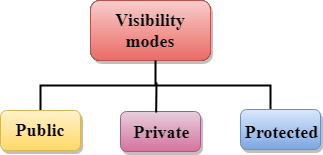
\includegraphics[width=\columnwidth]{visibillity-of-the-code}%
\caption{Visibiity modes}%
\label{}%
\end{figure}

\begin{enumerate}
	\item \textit{Public}: When the member is declared as public, it is accessible to all the functions of the program.
\item \textit{Private}: When the member is declared as private, it is accessible within the class only.
\item \textit{Protected}: When the member is declared as protected, it is accessible within its own class as well as the class immediately derived from it.
\end{enumerate}

Visibility of Inherited Members

\begin{table}
\centering
\small 
\begin{tabular}{l|lll} \hline \\
Base class visibility	& \multicolumn{3}{c}{Derived class visibility} \\ \hline 
& Public	& Private	& Protected \\ \hline 
Private	& Not Inherited	& Not Inherited	& Not Inherited \\
Protected	& Protected	& Private	& Protected \\
Public	& Public	& Private	& Protected \\ \hline 

\end{tabular}
\caption{Visibility of Inherited Members}
\end{table}
\normalsize

\subsection{C++ Multilevel Inheritance}

Multilevel inheritance is a process of deriving a class from another derived class.

\begin{figure}[h]

\includegraphics[width=\columnwidth]{multi-level-inheritance}%
\caption{Multilevel inheritance}%
\label{}%
\end{figure}

\subsubsection{C++ Multi Level Inheritance Example}

When one class inherits another class which is further inherited by another class, it is known as multi level inheritance in C++. Inheritance is transitive so the last derived class acquires all the members of all its base classes. Let's see the example of multi level inheritance in C++.

\begin{lstlisting}
#include <iostream>  
using namespace std;  
 class Animal {  
   public:  
 void eat() {   
    cout<<"Eating..."<<endl;   
 }    
   };  
   class Dog: public Animal   
   {    
       public:  
     void bark(){  
    cout<<"Barking..."<<endl;   
     }    
   };   
   class BabyDog: public Dog   
   {    
       public:  
     void weep() {  
    cout<<"Weeping...";   
     }    
   };   
int main(void) {  
    BabyDog d1;  
    d1.eat();  
    d1.bark();  
     d1.weep();  
     return 0;  
}  
\end{lstlisting}

Output:

\begin{verbatim}
Eating...
Barking...
Weeping...
\end{verbatim}

\begin{figure}[h]
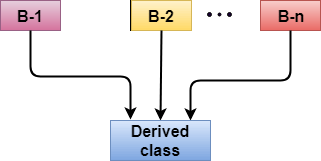
\includegraphics[width=\columnwidth]{multiple-inheritance}%
\caption{Multiple inheritance}%
\label{}%
\end{figure}

Multiple inheritance is the process of deriving a new class that inherits the attributes from two or more classes.

Syntax of the Derived class:

\begin{lstlisting}
class D : visibility B-1, visibility B-2, ?  
{  
    // Body of the class;  
}   
\end{lstlisting}

Let's see a simple example of multiple inheritance.

\begin{lstlisting}
#include <iostream>  
using namespace std;  
class A  
{  
    protected:  
     int a;  
    public:  
    void get_a(int n)  
    {  
        a = n;  
    }  
};  
  
class B  
{  
    protected:  
    int b;  
    public:  
    void get_b(int n)  
    {  
        b = n;  
    }  
};  
class C : public A,public B  
{  
   public:  
    void display()  
    {  
        std::cout << "The value of a is : " <<a<< std::endl;  
        std::cout << "The value of b is : " <<b<< std::endl;  
        cout<<"Addition of a and b is : "<<a+b;  
    }  
};  
int main()  
{  
   C c;  
   c.get_a(10);  
   c.get_b(20);  
   c.display();  
  
    return 0;  
}  
\end{lstlisting}

Output:

\begin{verbatim}
The value of a is : 10
The value of b is : 20
Addition of a and b is : 30

\end{verbatim}

In the above example, class 'C' inherits two base classes 'A' and 'B' in a public mode.

\subsection{Ambiquity Resolution in Inheritance}

Ambiguity can be occurred in using the multiple inheritance when a function with the same name occurs in more than one base class.

Let's understand this through an example:

\begin{lstlisting}
#include <iostream>  
using namespace std;  
class A  
{  
    public:  
    void display()  
    {  
        std::cout << "Class A" << std::endl;  
    }  
};  
class B  
{  
    public:  
    void display()  
    {  
        std::cout << "Class B" << std::endl;  
    }  
};  
class C : public A, public B  
{  
    void view()  
    {  
        display();  
    }  
};  
int main()  
{  
    C c;  
    c.display();  
    return 0;  
}  
\end{lstlisting}

Output:

\begin{verbatim}
error: reference to 'display' is ambiguous
        display();

\end{verbatim}

The above issue can be resolved by using the class resolution operator with the function. In the above example, the derived class code can be rewritten as:

\begin{lstlisting}
class C : public A, public B  
{  
    void view()  
    {  
        A :: display();         // Calling the display() function of class A.  
        B :: display();         // Calling the display() function of class B.  
  
    }  
};  
\end{lstlisting}

An ambiguity can also occur in single inheritance.

Consider the following situation:

\begin{lstlisting}
class A  
{  
   public:  
void display()  
{  
   cout<<?Class A?;  
}   
} ;  
class B  
{   
  public:  
 void display()  
{  
 cout<<?Class B?;  
}  
} ;  
\end{lstlisting}

In the above case, the function of the derived class overrides the method of the base class. Therefore, call to the display() function will simply call the function defined in the derived class. If we want to invoke the base class function, we can use the class resolution operator.

\begin{lstlisting}
int main()  
{  
    B b;  
   b.display();               // Calling the display() function of B class.  
   b.B :: display();       // Calling the display() function defined in B class.  
}   
\end{lstlisting}

\subsection{C++ Hybrid Inheritance}

Hybrid inheritance is a combination of more than one type of inheritance.

\begin{figure}[h]
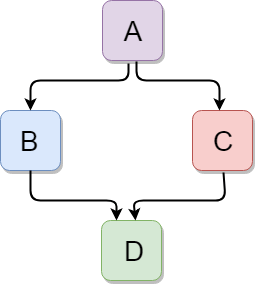
\includegraphics[width=\columnwidth]{hybrid-inheritance}%
\caption{Hybrid inheritance}%
\label{}%
\end{figure}

Let's see a simple example:

\begin{lstlisting}
#include <iostream>  
using namespace std;  
class A  
{  
    protected:  
    int a;  
    public:  
    void get_a()  
    {  
       std::cout << "Enter the value of 'a' : " << std::endl;  
       cin>>a;  
    }  
};  
  
class B : public A   
{  
    protected:  
    int b;  
    public:  
    void get_b()  
    {  
        std::cout << "Enter the value of 'b' : " << std::endl;  
       cin>>b;  
    }  
};  
class C   
{  
    protected:  
    int c;  
    public:  
    void get_c()  
    {  
        std::cout << "Enter the value of c is : " << std::endl;  
        cin>>c;  
    }  
};  
  
class D : public B, public C  
{  
    protected:  
    int d;  
    public:  
    void mul()  
    {  
         get_a();  
         get_b();  
         get_c();  
         std::cout << "Multiplication of a,b,c is : " <<a*b*c<< std::endl;  
    }  
};  
int main()  
{  
    D d;  
    d.mul();  
    return 0;  
}  
\end{lstlisting}

Output:

\begin{verbatim}
Enter the value of 'a' :
10              
Enter the value of 'b' :    
20      
Enter the value of c is :   
30  
Multiplication of a,b,c is : 6000

\end{verbatim}

\subsection{C++ Hierarchical Inheritance}

Hierarchical inheritance is defined as the process of deriving more than one class from a base class.

\begin{figure}[h]
\includegraphics[width=\columnwidth]{filename}%
\caption{Hierarchical inheritance}%
\label{}%
\end{figure}

Syntax of Hierarchical inheritance:

\begin{lstlisting}
class A  
{  
    // body of the class A.  
}    
class B : public A   
{  
    // body of class B.  
}  
class C : public A  
{  
    // body of class C.  
}   
class D : public A  
{  
    // body of class D.  
}   
\end{lstlisting}

Let's see a simple example:

\begin{lstlisting}
#include <iostream>  
using namespace std;  
class Shape                 // Declaration of base class.  
{  
    public:  
    int a;  
    int b;  
    void get_data(int n,int m)  
    {  
        a= n;  
        b = m;  
    }  
};  
class Rectangle : public Shape  // inheriting Shape class  
{  
    public:  
    int rect_area()  
    {  
        int result = a*b;  
        return result;  
    }  
};  
class Triangle : public Shape    // inheriting Shape class  
{  
    public:  
    int triangle_area()  
    {  
        float result = 0.5*a*b;  
        return result;  
    }  
};  
int main()  
{  
    Rectangle r;  
    Triangle t;  
    int length,breadth,base,height;  
    std::cout << "Enter the length and breadth of a rectangle: " << std::endl;  
    cin>>length>>breadth;  
    r.get_data(length,breadth);  
    int m = r.rect_area();  
    std::cout << "Area of the rectangle is : " <<m<< std::endl;  
    std::cout << "Enter the base and height of the triangle: " << std::endl;  
    cin>>base>>height;  
    t.get_data(base,height);  
    float n = t.triangle_area();  
    std::cout <<"Area of the triangle is : "  << n<<std::endl;  
    return 0;  
}  
\end{lstlisting}

Output:

\begin{verbatim}
Enter the length and breadth of a rectangle:
23  
20  
Area of the rectangle is : 460          
Enter the base and height of the triangle:  
2   
5
Area of the triangle is : 5 

\end{verbatim}

\section{C++ Polymorphism}

The term \enquote{Polymorphism} is the combination of \enquote{poly} + \enquote{morphs} which means many forms. It is a greek word. In object-oriented programming, we use 3 main concepts: inheritance, encapsulation, and polymorphism.

Let's consider a real-life example of polymorphism. A lady behaves like a teacher in a classroom, mother or daughter in a home and customer in a market. Here, a single person is behaving differently according to the situations.

There are two types of polymorphism in C++:

\begin{enumerate}
	\item \textit{Compile time polymorphism}: The overloaded functions are invoked by matching the type and number of arguments. This information is available at the compile time and, therefore, compiler selects the appropriate function at the compile time. It is achieved by function overloading and operator overloading which is also known as static binding or early binding. Now, let's consider the case where function name and prototype is same.

\begin{lstlisting}
   class A                                  //  base class declaration.  
  {  
       int a;  
       public:  
       void display()  
       {   
             cout<< "Class A ";  
        }  
  };  
class B : public A                       //  derived class declaration.  
{  
    int b;  
    public:  
   void display()  
  {  
        cout<<"Class B";  
  }  
};  
\end{lstlisting}

In the above case, the prototype of display() function is the same in both the base and derived class. Therefore, the static binding cannot be applied. It would be great if the appropriate function is selected at the run time. This is known as run time polymorphism.

\item \textit{Run time polymorphism}: Run time polymorphism is achieved when the object's method is invoked at the run time instead of compile time. It is achieved by method overriding which is also known as dynamic binding or late binding.

\end{enumerate}

\subsection{Differences b/w compile time and run time polymorphism.}

\begin{table} 
\tiny
\begin{tabular}{l|l} \hline \\
Compile time polymorphism	& Run time polymorphism \hline \\
The function to be invoked is known at the compile time.	& The function to be invoked is known at the run time. \\
It is also known as overloading, early binding and static binding.	& It is also known as overriding, Dynamic binding and late binding. \\
Overloading is a compile time polymorphism where more than one method is having the same name but with the different number of parameters or the type of the parameters.	& Overriding is a run time polymorphism where more than one method is having the same name, number of parameters and the type of the parameters. \\
It is achieved by function overloading and operator overloading.	& It is achieved by virtual functions and pointers. \\
It provides fast execution as it is known at the compile time.	& It provides slow execution as it is known at the run time. \\
It is less flexible as mainly all the things execute at the compile time.	& It is more flexible as all the things execute at the run time. \\ \hline 

\end{tabular}

\caption{Differences between compile time and runtime polymorphisms}

\end{table}
\normalsize

\subsubsection{C++ Runtime Polymorphism Example}

Let's see a simple example of run time polymorphism in C++.

\begin{lstlisting}
// an example without the virtual keyword.

#include <iostream>    
using namespace std;    
class Animal {    
    public:    
void eat(){      
cout<<"Eating...";      
    }        
};     
class Dog: public Animal      
{      
 public:    
 void eat()      
    {           cout<<"Eating bread...";      
    }      
};    
int main(void) {    
   Dog d = Dog();      
   d.eat();    
   return 0;    
}    
\end{lstlisting}

Output:

\begin{verbatim}
Eating bread...
\end{verbatim}

\subsubsection{C++ Run time Polymorphism Example: By using two derived class}

Let's see another example of run time polymorphism in C++ where we are having two derived classes.

\begin{lstlisting}
// an example with virtual keyword.

#include <iostream>    
using namespace std;    
class Shape {                                        //  base class  
    public:    
virtual void draw(){                             // virtual function  
cout<<"drawing..."<<endl;      
    }        
};     
class Rectangle: public Shape                  //  inheriting Shape class.  
{      
 public:    
 void draw()      
   {      
       cout<<"drawing rectangle..."<<endl;      
    }      
};    
class Circle: public Shape                        //  inheriting Shape class.  
  
{      
 public:    
 void draw()      
   {      
      cout<<"drawing circle..."<<endl;      
   }      
};    
int main(void) {    
    Shape *s;                               //  base class pointer.  
    Shape sh;                               // base class object.  
       Rectangle rec;    
        Circle cir;    
      s=&sh;    
     s->draw();     
        s=&rec;    
     s->draw();      
    s=?    
    s->draw();     
}    
\end{lstlisting}

Output:

\begin{verbatim}
drawing...
drawing rectangle...
drawing circle...
\end{verbatim}

\subsection{Runtime Polymorphism with Data Members}

Runtime Polymorphism can be achieved by data members in C++. Let's see an example where we are accessing the field by reference variable which refers to the instance of derived class.

\begin{lstlisting}
#include <iostream>    
using namespace std;    
class Animal {                                          //  base class declaration.  
    public:    
    string color = "Black";      
};     
class Dog: public Animal                       // inheriting Animal class.  
{      
 public:    
    string color = "Grey";      
};    
int main(void) {    
     Animal d= Dog();      
    cout<<d.color;     
}    
\end{lstlisting}

Output:

\begin{verbatim}
Black
\end{verbatim}

\begin{comment}
\newpage
\begin{multicols}{2}
\theendnotes
\end{multicols}
\end{comment}

\chapter{File Handling}

\section{What is file handling in C++?}

Files store data permanently in a storage device. With file handling, the output from a program can be stored in a file. Various operations can be performed on the data while in the file.

A stream is an abstraction of a device where input/output operations are performed. You can represent a stream as either a destination or a source of characters of indefinite length. This will be determined by their usage. C++ provides you with a library that comes with methods for file handling. Let us discuss it.

\section{The \texttt{fstream} Library}

The fstream library provides C++ programmers with three classes for working with files. These classes include:

\begin{enumerate}
	\item \textit{ofstream}: This class represents an output stream. It’s used for creating files and writing information to files.
\item \textit{ifstream}: This class represents an input stream. It’s used for reading information from data files.
\item \textit{fstream}: This class generally represents a file stream. It comes with ofstream/ifstream capabilities. This means it’s capable of creating files, writing to files, reading from data files.

\end{enumerate}

To use the above classes of the fstream library, you must include it in your program as a header file. Of course, you will use the \texttt{#include} preprocessor directive. You must also include the \texttt{iostream} header file.

\section{How to Open Files}

Before performing any operation on a file, you must first open it. If you need to write to the file, open it using \texttt{fstream} or \texttt{ofstream} objects. If you only need to read from the file, open it using the \texttt{ifstream} object.

The three objects, that is, \texttt{fstream, ofstream}, and \texttt{ifstream}, have the \texttt{open()} function defined in them. The function takes this syntax:

\begin{lstlisting}
open (file_name, mode);
\end{lstlisting}

\begin{enumerate}
	\item The \texttt{file\_name} parameter denotes the name of the file to open.
\item The mode parameter is optional. It can take any of the following values:
\end{enumerate}

\begin{table}
\tiny
\begin{tabular}{ll} \hline \\
Value	& Description \\ \hline 
\texttt{ios::app}	& The Append mode. The output sent to the file is appended to it. \\
\texttt{ios::ate}	& It opens the file for the output then moves the read and write control to file’s end. \\
\texttt{ios::in}	& It opens the file for a read. \\
\texttt{ios::out}	& It opens the file for a write. \\
\texttt{ios::trunc}	& If a file exists, the file elements should be truncated prior to its opening. \\ \hline
\end{tabular}
\end{table}
\normalsize

It is possible to use two modes at the same time. You combine them using the \textit{| (OR)} operator.

\subsection{Example 1}

\begin{lstlisting}
#include <iostream>
#include <fstream>
using namespace std;
int main() {
	fstream my_file;
	my_file.open("my_file", ios::out);
	if (!my_file) {
		cout << "File not created!";
	}
	else {
		cout << "File created successfully!";
		my_file.close(); 
	}
	return 0;
}
\end{lstlisting}

\section{How to Close Files}

Once a C++ program terminates, it automatically

\begin{enumerate}
	\item flushes the streams
\item releases the allocated memory
\item closes opened files.
\end{enumerate}

However, as a programmer, you should learn to close open files before the program terminates.

The \texttt{fstream, ofstream}, and \texttt{ifstream} objects have the \texttt{close() }function for closing files. The function takes this syntax:

\begin{lstlisting}
void close();
\end{lstlisting}

\section{Write to Files}

You can write to file right from your C++ program. You use stream insertion operator \texttt{(<<)} for this. The text to be written to the file should be enclosed within double-quotes.

Let us demonstrate this.

\subsection{Example 2}

\begin{lstlisting}
#include <iostream>
#include <fstream>
using namespace std;
int main() {
	fstream my_file;
	my_file.open("my_file.txt", ios::out);
	if (!my_file) {
		cout << "File not created!";
	}
	else {
		cout << "File created successfully!";
		my_file << "Hello World!";
		my_file.close();
	}
	return 0;
}
\end{lstlisting}

\section{Read from Files}

You can read information from files into your C++ program. This is possible using stream extraction operator \texttt{(>>)}. You use the operator in the same way you use it to read user input from the keyboard. However, instead of using the cin object, you use the ifstream/ fstream object.

\subsection{Example 3}

\begin{lstlisting}
#include <iostream>
#include <fstream>
using namespace std;
int main() {
	fstream my_file;
	my_file.open("my_file.txt", ios::in);
	if (!my_file) {
		cout << "No such file";
	}
	else {
		char ch;

		while (1) {
			my_file >> ch;
			if (my_file.eof())
				break;

			cout << ch;
		}

	}
	my_file.close();
	return 0;
}
\end{lstlisting}

\chapter{Exception Handling}

Exception Handling in C++ is a process to handle \textit{runtime} errors. We perform exception handling so the normal flow of the application can be maintained even after \textit{runtime} errors.

In C++, exception is an event or object which is thrown at runtime. All exceptions are derived from \texttt{std::exception} class. It is a runtime error which can be handled. If we don't handle the exception, it prints exception message and terminates the program. The main advantage is that it maintains the normal flow of the application. In such case, rest of the code is executed even after exception.

\section{C++ Exception Classes}

In C++ standard exceptions are defined in \texttt{<exception>} class that we can use inside our programs. The arrangement of parent-child class hierarchy is shown below:

\subsection{Accessing Elements of Union}

\begin{figure}[h]
\centering 
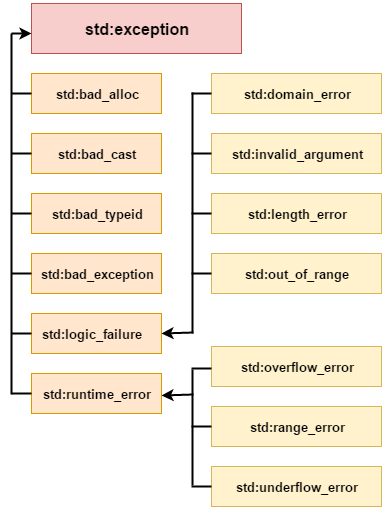
\includegraphics[width=6cm, height=7cm]{cpp-exception-handling}%
\caption{Errors and Exceptions}%
\label{}%
\end{figure}

All the exception classes in C++ are derived from std::exception class. Let's see the list of C++ common exception classes.

\begin{table}
\tiny
\begin{tabular}{ll} \hline \\
Exception	& Description \hline \\
\texttt{std::exception}	& It is an exception and parent class of all standard C++ exceptions. \\
\texttt{std::logic\_failure}	& It is an exception that can be detected by reading a code. \\
\texttt{std::runtime\_error}	& It is an exception that cannot be detected by reading a code. \\
\texttt{std::bad\_exception}	& It is used to handle the unexpected exceptions in a c++ program. \\
\texttt{std::bad\_cast}	& This exception is generally be thrown by $dynamic\_cast$. \\
\texttt{std::bad\_typeid}	& This exception is generally be thrown by \texttt{typeid}. \\
\texttt{std::bad\_alloc}	& This exception is generally be thrown by new. \\ \hline 

\end{tabular}
\end{table}

\subsection{C++ Exception Handling Keywords}

In C++, we use 3 keywords to perform exception handling:

\begin{enumerate}
	\item try
\item catch, and
\item throw
\end{enumerate}

Moreover, we can create user-defined exception which we will learn in next chapters.

\section{C++ try/catch}

In C++ programming, exception handling is performed using try/catch statement. The C++ try block is used to place the code that may occur exception. The catch block is used to handle the exception.

\subsection{C++ example without try/catch}

\begin{lstlisting}
#include <iostream>  
using namespace std;  
float division(int x, int y) {  
   return (x/y);  
}  
int main () {  
   int i = 50;  
   int j = 0;  
   float k = 0;  
      k = division(i, j);  
      cout << k << endl;  
   return 0;  
}  
\end{lstlisting}

Output:

\begin{verbatim}
Floating point exception (core dumped)  
\end{verbatim}
 
\subsubsection{C++ try/catch example}

\begin{lstlisting}
#include <iostream>  
using namespace std;  
float division(int x, int y) {  
 if( y == 0 ) {  
	throw "Attempted to divide by zero!";  
 }  
 return (x/y);  
}  
int main () {  
   int i = 25;  
   int j = 0;  
   float k = 0;  
   try {  
      k = division(i, j);  
      cout << k << endl;  
   }catch (const char* e) {  
      cerr << e << endl;  
   }  
   return 0;  
}  
\end{lstlisting}

Output:

\begin{verbatim}
Attempted to divide by zero!
\end{verbatim}

\section{C++ User-Defined Exceptions}

The new exception can be defined by overriding and inheriting exception class functionality.

\subsection{C++ user-defined exception example}

Let's see the simple example of user-defined exception in which std::exception class is used to define the exception.

\begin{lstlisting}
#include <iostream>  
#include <exception>  
using namespace std;  
class MyException : public exception{  
	public:  
		const char * what() const throw()  
		{  
			return "Attempted to divide by zero!\n";  
		}  
};  
int main()  
{  
	try  
	{  
		int x, y;  
		cout << "Enter the two numbers : \n";  
		cin >> x >> y;  
		if (y == 0)  
		{  
				MyException z;  
				throw z;  
		}  
		else  
		{  
				cout << "x / y = " << x/y << endl;  
		}  
	}  
	catch(exception& e)  
	{  
		cout << e.what();  
	}  
}  
\end{lstlisting}

Output:

\begin{verbatim}
Enter the two numbers :
10
2
x / y = 5  

\end{verbatim}

Output:

\begin{verbatim}
Enter the two numbers :
10
0
Attempted to divide by zero!

\end{verbatim}

\section{Built-in Exceptions}

\subsection{\texttt{bad\_alloc} exception}

Standard C++ contains several built-in exception classes. The most commonly used is $bad\_alloc$, which is thrown if an error occurs when attempting to allocate memory with new. This class is derived from exception. To make use of $bad\_alloc$, one should set up the appropriate try and catch blocks. Here’s a short example, that shows how it’s used :

\begin{lstlisting}
// CPP code for bad_alloc
#include <iostream>
#include <new>
  
// Driver code
int main () {
  try
  {
     int* gfg_array = new int[100000000];
  }
  catch (std::bad_alloc & ba)
  {
     std::cerr << "bad_alloc caught: " << ba.what();
  }
  return 0;
}
\end{lstlisting}

Output 

\begin{verbatim}
RunTime error :
bad_alloc caught: std::bad_alloc
\end{verbatim}

\subsection{\texttt{bad\_cast} exception}

Standard C++ contains several built-in exception classes. \texttt{typeinfo::bad\_cast} is one of them. This is an exception thrown on failure to dynamic cast. Below is the syntax for the same:

Header File:

\begin{verbatim}
<typeinfo>
\end{verbatim}

Syntax:

\begin{verbatim}
class bad_cast;
\end{verbatim}

To make use of \texttt{std::bad\_cast}, one should set up the appropriate try and catch blocks. It doesn't return anything. Below are the examples to understand the implementation of std::bad_cast in a better way:

Program 1:

\begin{lstlisting}
// C++ code for std::bad_cast
#include <bits/stdc++.h>
#include <typeinfo>
  
using namespace std;
  
// Base Class
class Base {
    virtual void member() {}
};
  
// Derived Class
class Derived : Base {
};
  
// main() method
int main()
{
  
    // try block
    try {
        Base gfg;
        Derived& rd
            = dynamic_cast<Derived&>(gfg);
    }
  
    // catch block to handle the errors
    catch (bad_cast& bc) {
        cerr << "bad_cast caught: "
             << bc.what() << endl;
    }
  
    return 0;
}
\end{lstlisting}
Output:

\begin{verbatim}
bad_cast caught: std::bad_cast
\end{verbatim}

Program 2:

\begin{lstlisting}
// C++ code for std::bad_cast
#include <bits/stdc++.h>
#include <typeinfo>
  
using namespace std;
  
// Base Class
class Base {
    virtual void member() {}
};
  
// Derived Class
class Derived : Base {
};
  
// main() method
int main()
{
  
    // try block
    try {
        Base geeksforgeeks;
        Derived& abc
            = dynamic_cast<Derived&>(
                geeksforgeeks);
    }
  
    // catch block to handle the errors
    catch (bad_cast& a) {
        cerr << "bad_cast caught: "
             << a.what() << endl;
    }
  
    return 0;
}
\end{lstlisting}
Output:

\begin{verbatim}
bad_cast caught: std::bad_cast
\end{verbatim}

\subsection{\texttt{bad\_typeid} exception}

Standard C++ contains several built-in exception classes, \texttt{typeinfo::bad\_typeid} is one of them. This is an exception thrown on typeid of null pointer. Below is the syntax for the same:

Header File:

\begin{verbatim}
<typeinfo>
\end{verbatim}

Syntax:

\begin{verbatim}
class bad_typeid;
\end{verbatim}

The \texttt{typeinfo::bad\_typeid} returns a null terminated character that is used to identify the exception. To make use of \texttt{std::bad\_typeid}, one should set up the appropriate try and catch blocks. Below are the examples to understand the implementation of \texttt{typeinfo::bad\_typeid} in a better way:

Program 1:

\begin{lstlisting}
// C++ code for std::bad_typeid
#include <bits/stdc++.h>
  
using namespace std;
  
struct gfg {
    virtual void func();
};
  
// main method
int main()
{
    gfg* g = nullptr;
  
    // try block
    try {
        cout << typeid(*g).name()
             << endl;
    }
  
    // catch block to handle the errors
    catch (const bad_typeid& fg) {
        cout << fg.what() << endl;
    }
  
    return 0;
}
\end{lstlisting}

Output:

\begin{verbatim}
std::bad_typeid
\end{verbatim}

Program 2:

\begin{lstlisting}
// C++ code for std::bad_typeid
#include <bits/stdc++.h>
  
using namespace std;
  
struct geeksforgeeks {
    virtual void
    A_Computer_Science_Portal_For_Geeks();
};
  
// main method
int main()
{
    geeksforgeeks* gfg = nullptr;
  
    // try block
    try {
        cout << typeid(*gfg).name() << endl;
    }
  
    // catch block to handle the errors
    catch (const bad_typeid& fg) {
        cout << fg.what() << endl;
    }
  
    return 0;
}
\end{lstlisting}

Output:

\begin{verbatim}
std::bad_typeid
\end{verbatim}

\subsection{\texttt{bad\_exception} exception}

Standard C++ contains several built-in exception classes, \texttt{exception::bad\_exception} is one of them. This is an exception thrown by unexpected handler. Below is the syntax for the same:

Header File:

\begin{verbatim}
include<exception>
\end{verbatim}

Syntax:

\begin{verbatim}
class bad_exception;
\end{verbatim}

The \texttt{exception::bad\_exception} returns a null terminated character that is used to identify the exception. To make use of \texttt{exception::bad\_exception}, one should set up the appropriate try and catch blocks. Below are the examples to understand the implementation of \texttt{exception::bad\_exception} in a better way:

Program 1 :

\begin{lstlisting}
// C++ code for std::bad_exception
#include <bits/stdc++.h>
  
using namespace std;
  
void func()
{
    throw;
}
  
void geeksforgeeks() throw(bad_exception)
{
    throw runtime_error("test");
}
  
// main method
int main()
{
    set_unexpected(func);
  
    // try block
    try {
        geeksforgeeks();
    }
  
    // catch block to handle the errors
    catch (const bad_exception& gfg) {
        cout << "Caught exception "
             << gfg.what() << endl;
    }
    return 0;
}
\end{lstlisting}

Output:

\begin{verbatim}
Caught exception std::bad_exception
\end{verbatim}

Program 2 :

\begin{lstlisting}
// C++ code for std::bad_exception
#include <bits/stdc++.h>
  
using namespace std;
  
void gfg()
{
    throw;
}
  
void A_Computer_Science_Portal_For_Geeks()
     throw(bad_exception)
{
    throw runtime_error("test");
}
  
// main method
int main()
{
    set_unexpected(gfg);
  
    // try block
    try {
        A_Computer_Science_Portal_For_Geeks();
    }
  
    // catch block to handle the errors
    catch (const bad_exception& a) {
        cout << "Caught exception "
             << a.what() << endl;
    }
    return 0;
}
\end{lstlisting}

Output:

\begin{verbatim}
Caught exception std::bad_exception
\end{verbatim}

\subsection{\texttt{logic\_error} exception}

The class serves as the base class for all exceptions thrown to report errors presumably detectable before the program executes, such as violations of logical preconditions.

Syntax

\begin{verbatim}
class logic_error : public exception {
public:
    explicit logic_error(const string& message);

    explicit logic_error(const char *message);

};
\end{verbatim}

Remarks

The value returned by what() is a copy of message.data(). For more information, see what and data.

Example 

\begin{lstlisting}
// logic_error.cpp
// compile with: /EHsc
#include <exception>
#include <iostream>
#include <stdexcept>
#include <typeinfo>
using namespace std;

int main()
{
   try
   {
      throw logic_error("Does not compute!");
   }
   catch (const exception& e)
   {
      cerr << "Caught: " << e.what() << endl;
      cerr << "Type: " << typeid(e).name() << endl;
   }
}
/* Output:
Caught: Does not compute!
Type: class std::logic_error
*/
\end{lstlisting}

\section{Runtime error}

In this article, we will discuss the reason for the run-time error and its solution. A \textit{runtime error} in a program is an error that occurs while the program is running after being successfully compiled. Below are some methods to identify the reason behind Runtime error:

\subsection{Invalid memory access}

When the index of the array is assigned with a negative index it leads to invalid memory access during runtime error. Below is the C++ Program to illustrate the invalid memory access during run-time:

\begin{lstlisting}
// C++ program to illustrate invalid
// memory access during run-time
#include <iostream>
using namespace std;
  
// Global declaration
int arr[5];
  
// Driver Code
int main()
{
    int answer = arr[-10];
    cout << answer;
  
    return 0;
}
\end{lstlisting}

Output:

\begin{verbatim}
1736487104
\end{verbatim}

\subsection{Array runs out of bound}

Sometimes Array or vector runs out of bound of their limits resulting in a runtime error. Below is the C++ program illustrating array runs out of bound:

\begin{lstlisting}
// C++ program to illustrate
// array runs out of bound
#include <iostream>
using namespace std;
  
// Driver Code
int main()
{
    long n;
    n = 100000000000;
  
    // 'n' is out of bound for
    // the array limit
    long a[n];
  
    cout << a[1] << " ";
    return 0;
}
\end{lstlisting}

It can be resolved by using the size of the array/vector as within the limit. 

\subsection{Unassigned variables}

Some silly mistakes encountered while coding in hurry, sometimes leads to runtime error. Below is the C++ program illustrating runtime error by un-assigned variables:

\begin{lstlisting}
// C++ program to illustrate runtime
// error by un-assigned variables
#include <iostream>
using namespace std;
  
// Driver Code
int main()
{
    long long N;
  
    // N is assigned garbage value
    long arr[N];
  
    cin >> N;
  
    for (int i = 0; i < N; i++) {
        cin >> arr[i];
    }
  
    for (int i = 0; i < N; i++) {
        cout << arr[i] << " ";
    }
  
    return 0;
}
\end{lstlisting}


Here, variable \textit{N} is assigned a garbage value resulting in a runtime error. Sometimes, since it depends on the compiler how it assigned the garbage value. This can be resolved by declaring \textit{arr[N]} after scanning the value for variable n and checking if it is the upper or lower limit of the array/vector index.




\end{document}